\documentclass{article}
\usepackage{polski}
\usepackage{graphicx}
\usepackage{amsmath}
\usepackage{hyperref}
\usepackage{float}
\usepackage{algorithm}
\usepackage{subcaption}
\graphicspath{ {./images/} }
\hypersetup{%
	pdfborder = {0 0 0}
}

\author{Szymon Woźniak, 235040}
\date{16.05.2019}
\title{Podobieństwo obrazów}


\begin{document}
	\pagenumbering{gobble}
	\maketitle
	\newpage
	\pagenumbering{arabic}
	
	\section{Wstęp teoretyczny}
	\subsection{Cel zadania}
	Celem zadania jest określania podobieństwa obrazów poprzez poszukiwanie obiektów występujących na obu.
	
	\subsection{Punkty kluczowe}
	Punkty kluczowe opisują lokalną charakterystykę wizualną danego obrazu. Każdy punkt kluczowy opisany jest wektorem cech. Do celów zadania zostanie użyty gotowe narzędzie do ekstrakcji cech, korzystający z detektora Harris-Affine i deskryptora SIFT.
	\subsection{Wyznaczanie par punktów kluczowych}
	Do wyznaczania par punktów kluczowych zastosowany zostanie użyty algorytm wzajemnego najbliższego sąsiada. Dla każdego punktu z jednego z obrazów zostaje wyznaczony punkt z drugiego obrazu będący najbliższy do niego w sensie podobieństwa cech. Ta sama procedura jest przeprowadzana dla punktów z drugiego obrazu. Para punktów (P, Q) zostaje utworzona tylko wtedy, gdy najbliższym punktem dla punktu P jest punkt Q, a najbliższym dla punktu Q jest punkt P. Funkcja odległości używana do porównywania punktów kluczowych ma postać:
	\begin{equation}
		distance(P, Q) = \sum_{i=1}^{n} |features(P, i) - features(Q, i)|,
	\end{equation}
	gdzie:
	\begin{itemize}
		\item n jest liczbą cech punktu kluczowego,
		\item features(R, i) jest wartość i-tej cechy z punktu R.
	\end{itemize}
	\subsection{Algorytm analizy spójności sąsiedztwa}
	Pary punktów kluczowych wyznaczanych przy pomocy algorytmu wzajemnego najbliższego sąsiada nie są wystarczające do wyznaczania podobieństwa obrazów. Jest tak ponieważ znacząca liczba znajdowanych par stanowi szum informacyjny.\\
	Do odfiltrowania nieznaczących par można wykorzystać algorytm analizy spójności sąsiedztwa. Algorytm ten na wejściu przyjmuje zbiór par znalezionych na obrazach. Zachowywane są  tylko te pary, które spełniają założone kryterium spójności.
	Najpierw dla każdego punktu na obu obrazach wyznaczane zostaje jego sąsiedztwo. Sąsiedztwem nazywany jest zbiór punktów o wielkości $k$, z tego samego obrazu, których odległość od zadanego punktu jest najmniejsza i większa od 0.\\
	Para punktów kluczowych $(Q_i, Q_j)$ sąsiaduje z parą punktów $(P_i, P_j)$ jeżeli punkt $Q_i$ należy do sąsiedztwa punktu $P_i$, a punkt $Q_j$ należy do sąsiedztwa punktu $P_j$.
	Sąsiedztwo pary punktów kluczowych jest nazywane \textbf{spójnym} jeżeli, para punktów kluczowych sąsiaduje z co najmniej $n$ innych par punktów kluczowych.
	\subsection{Metoda Random Sample Consensus}
	Metoda Random Sample Consensus("RANSAC") jest metodą pseudolosową służącą do estymacji parametrów modelu uczenia maszynowego. Jest ona zdolna wyznaczać parametry modelu nawet dla danych o dużej liczbie danych odstających.
	Na początku metoda losuje z całego zbioru danych $D$ minimalną próbkę danych pozwalającą na przeprowadzenie uczenia. W kolejnym kroku przeprowadza się uczenie. Na koniec oceniana jest jakość modelu. Każda obserwacja sprawdzana jest pod kątem zgodności z modelem. Jeżeli wartość błędu nie przekracza zadanego progu, to mówi się że dana obserwacja jest zgodna z modelem. Obserwacje zgodne tworzą \textbf{konsensus}, a jego rozmiar oddaje ogólną jakość modelu. W metodzie RANSAC przeprowadzanych jest $i$ iteracji opisanych wcześniej, a wynikiem działania jest model posiadający największy konsensus. W opisywanym jako modele użyte zostaną dwa opisane poniżej przekształcenia geometryczne.
	\subsubsection{Model - transformata afiniczna}
	\textbf{Transformata afiniczna} jest złożeniem trzech przekształceń elementarnych - obrót, skalowanie i translacja. Może zostać wyznaczona przy użyciu trzech par punktów kluczowych w następujący sposób:
	\begin{equation}
	\left[\begin{matrix}
	a \\
	b \\
	c \\
	d \\
	e \\
	f \\
	\end{matrix}\right]
	=
	\left[\begin{matrix}
	x_1 & y_1 & 1 & 0 & 0 & 0 \\
	x_2 & y_2 & 1 & 0 & 0 & 0 \\
	x_3 & y_3 & 1 & 0 & 0 & 0 \\
	0 & 0 & 0 & x_1 & y_1 & 1 \\
	0 & 0 & 0 & x_2 & y_2 & 1 \\
	0 & 0 & 0 & x_3 & y_3 & 1 \\
	\end{matrix}\right]^{-1}
	\left[\begin{matrix}
	u_1 \\
	u_2 \\
	u_3 \\
	v_1 \\
	v_2 \\
	v_3 \\
	\end{matrix}\right]
	\end{equation}
	\begin{equation}
	\textbf{A} =\left[\begin{matrix}
	a & b & c \\
	d & e & f \\
	0 & 0 & 1
	\end{matrix} \right]
	\end{equation}
	\subsubsection{Model - transformata perspektywiczna}
	Transformata perspektywiczna rozszerza transformatę afiniczną o efekt rozciągnięcia/spłaszczenia wynikający z perspektywy. Można ją wyznaczyć przy pomocy 4 par punktów kluczowych według  poniższych równań:
	 \begin{equation}
	\left[\begin{matrix}
	a \\
	b \\
	c \\
	d \\
	e \\
	f \\
	g \\
	h \\
	\end{matrix}\right]
	=
	\left[\begin{matrix}
	x_1 & y_1 & 1 & 0 & 0 & 0 & -u_1x_1 & -u_1y_1 \\
	x_2 & y_2 & 1 & 0 & 0 & 0 & -u_2x_2 & -u_2y_2 \\
	x_3 & y_3 & 1 & 0 & 0 & 0 & -u_3x_3 & -u_3y_3 \\
	x_4 & y_4 & 1 & 0 & 0 & 0 & -u_4x_4 & -u_4y_4 \\
	0 & 0 & 0 &  x_1 & y_1 & 1 & -v_1x_1 & -v_1y_1 \\
	0 & 0 & 0 &  x_2 & y_2 & 1 & -v_2x_2 & -v_2y_2 \\
	0 & 0 & 0 &  x_3 & y_3 & 1 & -v_3x_3 & -v_3y_3 \\
	0 & 0 & 0 &  x_4 & y_4 & 1 & -v_4x_4 & -v_4y_4 \\
	\end{matrix}\right]^{-1}
	\left[\begin{matrix}
	u_1 \\
	u_2 \\
	u_3 \\
	u_4 \\
	v_1 \\
	v_2 \\
	v_3 \\
	v_4 \\
	\end{matrix}\right]
	\end{equation}
	\begin{equation}
	\textbf{H} =\left[\begin{matrix}
	a & b & c \\
	d & e & f \\
	g & h & 1
	\end{matrix} \right]
	\end{equation}
	\subsection{Heurystyki przyspieszające metodę RANSAC}
	\subsubsection{Heurystyki odległości par punktów}
	Ta heurystyka mówi, że jako próbka do algorytmu RANSAC powinny być wybierane punkty leżące stosunkowo blisko siebie. Ograniczeniem może być na przykład to, że odległość pomiędzy każdą parą wybranych punktów powinna być większa niż $1\%$ i mniejsza niż $30\%$ wielkości obrazu.
	\subsubsection{Heurystyka modyfikacji rozkładu}
	Ta heurystyka mówi, że rozkład prawdopodobieństwa wyboru par punktów kluczowych powinien być modyfikowany w trakcie działania metody. Pary punktów, które uzyskiwały większe rozmiary konsensusu powinny być losowane z większym prawdopodobieństwem.
	\subsubsection{Heurystyka liczby iteracji}
	W podstawowej wersji metody RANSAC liczba iteracji jest stała i musi zostać podana przez użytkownika. Jeżeli jednak podana liczba iteracji będzie zbyt duża w stosunku  do trudności problemu, to od pewnego momentu metoda może nie generować już lepszych modeli. Liczbę iteracji można jednak oszacować zgodnie ze wzorem: 
	\begin{equation}
		k = \frac{log\left(1 - p\right)}{log\left(1 - w^n\right)}
	\end{equation}
	, gdzie: 
	\begin{itemize}
		\item $p$ - prawdopodobieństwo, że po oszacowanej liczbie iteracji model jest dostatecznie dobrym przybliżeniem danych,
		\item $w$ - prawdopodobieństwo, że wylosowana para nie jest szumem,
		\item $n$ - liczba par potrzebnych do wyznaczenia parametrów transformaty (3 lub 4),
		\item $k$ - szacowana liczba iteracji.
	\end{itemize}
	Prawdopodobieństwo $p$ musi zostać zadane przez użytkownika. Prawdopodobieństwo $w$ może zostać oszacowane jako stosunek liczby par przed i po zastosowaniu algorytmu analizy spójności sąsiedztwa.
	\section{Badania}
	\subsection{Wykorzystane pary obrazów}
	\begin{figure}[H]
		\centering
		\begin{subfigure}[b]{0.4\linewidth}
			\includegraphics[width=\linewidth]{hp11.png}
		\end{subfigure}
		\begin{subfigure}[b]{0.4\linewidth}
			\includegraphics[width=\linewidth]{hp12.png}
		\end{subfigure}
		\caption{Książka "Harry Potter i Kamień Filozoficzny" w dwóch różnych ujęciach.}
		\label{fig:hp1}
	\end{figure}
	\begin{figure}[H]
		\centering
		\begin{subfigure}[b]{0.4\linewidth}
			\includegraphics[width=\linewidth]{hp21.png}
		\end{subfigure}
		\begin{subfigure}[b]{0.4\linewidth}
			\includegraphics[width=\linewidth]{hp22.png}
		\end{subfigure}
		\caption{Książka Harry Potter i Przeklęte Dziecko w dwóch różnych ujęciach.}
		\label{fig:hp2}
	\end{figure}
	\begin{figure}[H]
		\centering
		\begin{subfigure}[b]{0.4\linewidth}
			\includegraphics[width=\linewidth]{martin11.png}
		\end{subfigure}
		\begin{subfigure}[b]{0.4\linewidth}
			\includegraphics[width=\linewidth]{martin12.png}
		\end{subfigure}
		\caption{Książka "Brudne Gry" w dwóch różnych ujęciach.}
		\label{fig:martin}
	\end{figure}
	\begin{figure}[H]
		\centering
		\begin{subfigure}[b]{0.4\linewidth}
			\includegraphics[width=\linewidth]{k1.png}
		\end{subfigure}
		\begin{subfigure}[b]{0.4\linewidth}
			\includegraphics[width=\linewidth]{k2.png}
		\end{subfigure}
		\caption{Kubek w dwóch różnych ujęciach.}
		\label{fig:kubek}
	\end{figure}
	\begin{figure}[H]
		\centering
		\begin{subfigure}[b]{0.4\linewidth}
			\includegraphics[width=\linewidth]{house1.png}
		\end{subfigure}
		\begin{subfigure}[b]{0.4\linewidth}
			\includegraphics[width=\linewidth]{house2.png}
		\end{subfigure}
		\caption{Ossolineum w dwóch różnych ujęciach.}
		\label{fig:ossolineum}
	\end{figure}
	\subsection{Skuteczność algorytmu analizy spójności sąsiedztwa}
	Wyniki badań skuteczność algorytmu spójności sąsiedztwa zostaną przedstawione jako porównanie dwóch par obrazów z naniesionymi parami punktów kluczowych. Jedna para będzie reprezentować wszystkie znalezione pary, a druga pary po zastosowaniu algorytmu analizy spójności sąsiedztwa. Do przeprowadzenia tych badań wykorzystane zostaną zdjęcia z rysunku \ref{fig:ossolineum}.\\
	\begin{figure}[H]
		\centering
		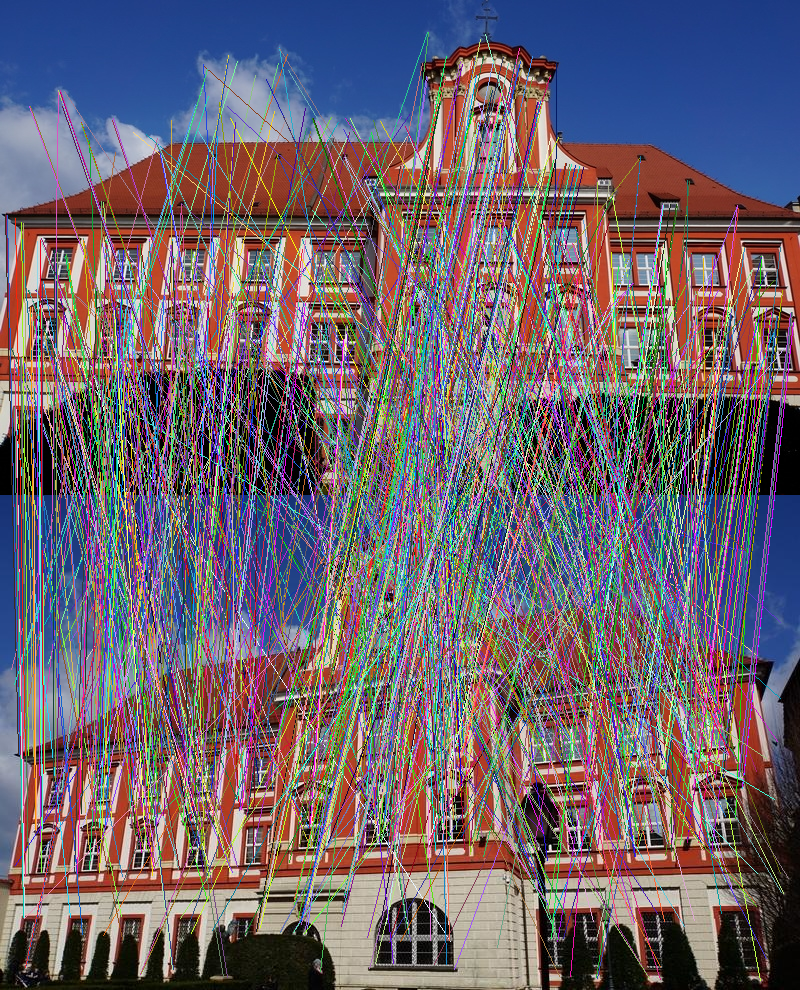
\includegraphics[width=0.6\linewidth]{1allpairs.png}
		\caption{Wszystkie pary punktów kluczowych znalezione na obrazach Ossolineum}
	\end{figure}
	\subsubsection{Wpływ wielkości sąsiedztwa na skuteczność algorytmu spójności}
	Wielkość sąsiedztwa została zbadana przy wartości progu spójności ustawionej na 0.5.
	\begin{figure}[H]
		\centering
		\begin{subfigure}[b]{0.4\linewidth}
			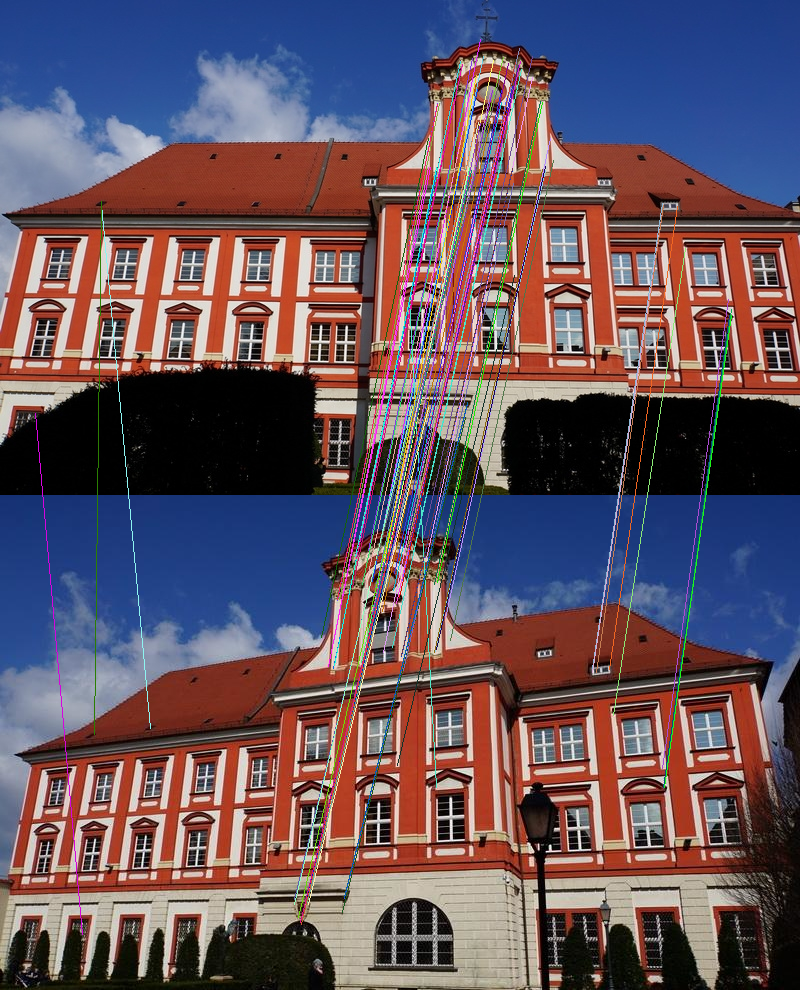
\includegraphics[width=\linewidth]{s50.png}
			\caption{n=50}
		\end{subfigure}
		\begin{subfigure}[b]{0.4\linewidth}
			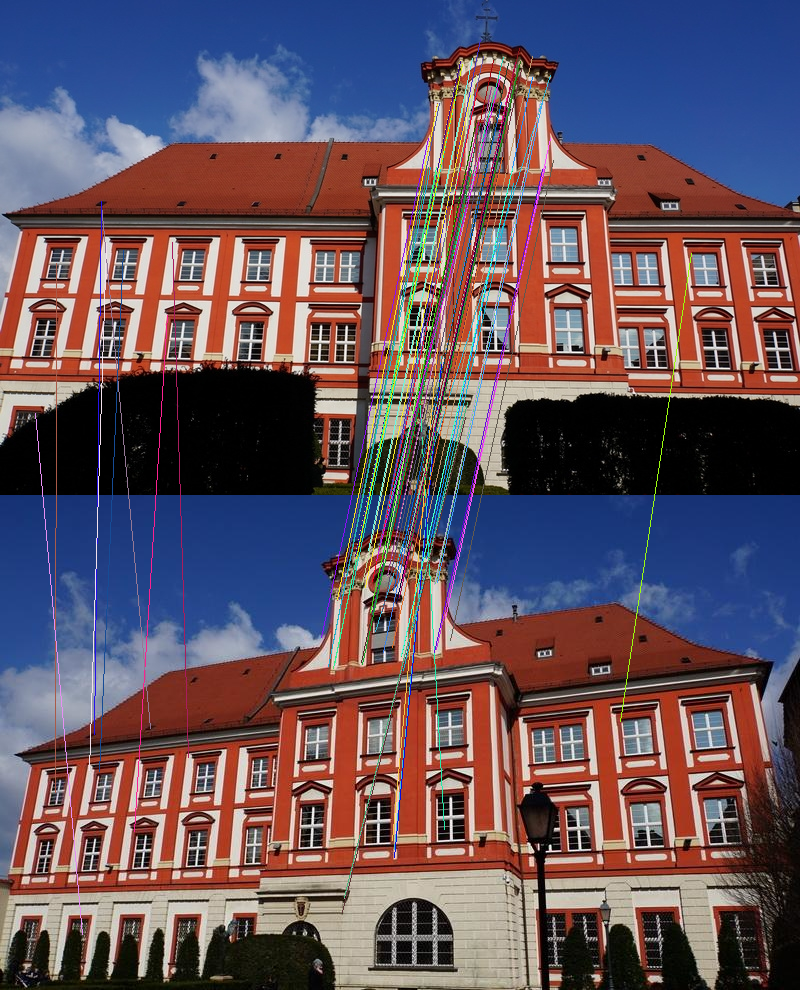
\includegraphics[width=\linewidth]{s100.png}
			\caption{n=100}
		\end{subfigure}
		\begin{subfigure}[b]{0.4\linewidth}
			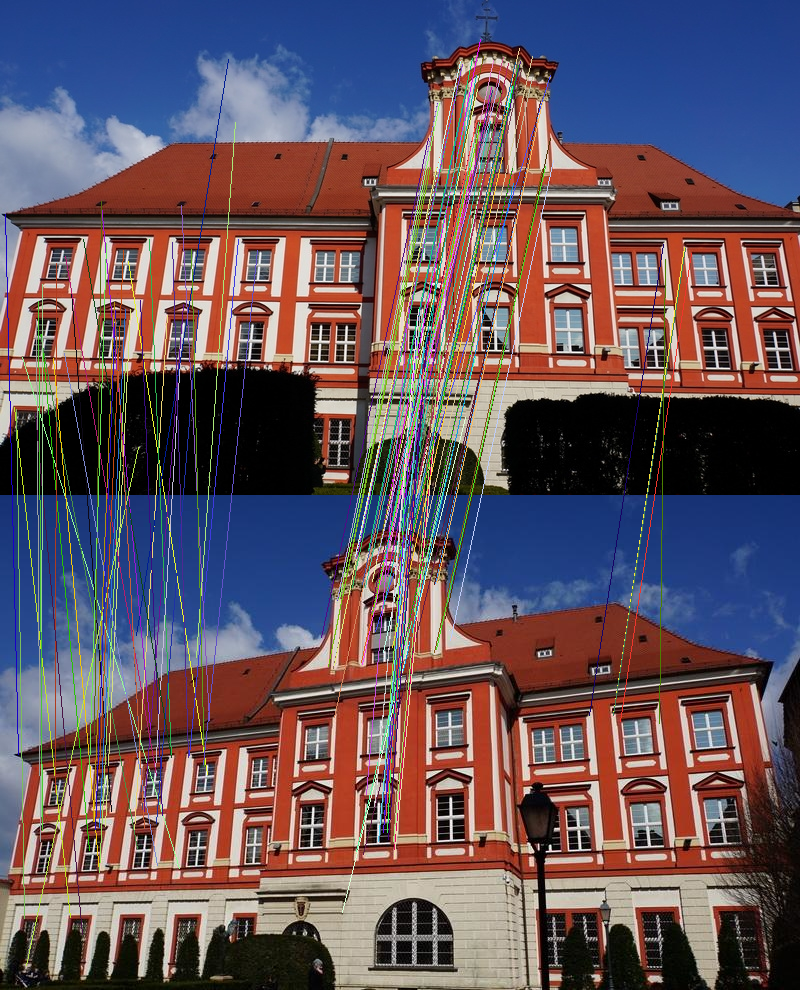
\includegraphics[width=\linewidth]{s150.png}
			\caption{n=150}
		\end{subfigure}
		\begin{subfigure}[b]{0.4\linewidth}
			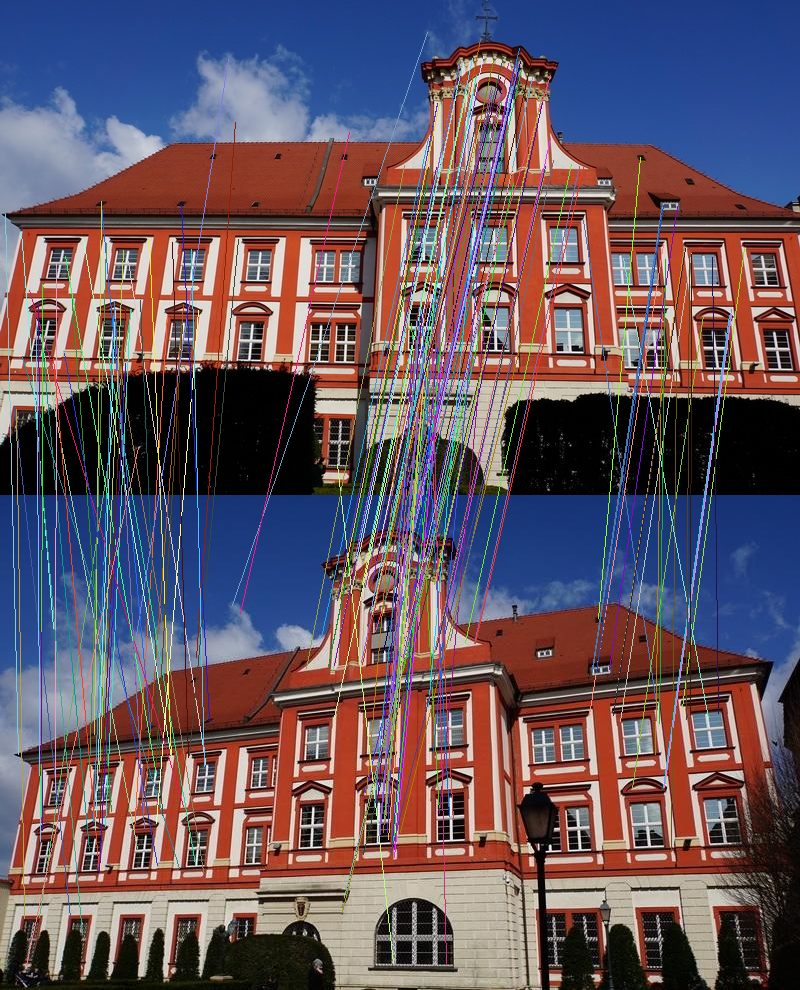
\includegraphics[width=\linewidth]{s200.png}
			\caption{n=200}
		\end{subfigure}
		\caption{Pary punktów kluczowych odfiltrowane za pomocą algorytmu spójności sąsiedztwa dla różnych wartości wielkości sąsiedztwa.}
		\label{fig:nsize}
	\end{figure}

	\begin{table}[H]
		\centering
		\caption{Porównanie liczby zaakceptowanych par punktów kluczowych i czasu przetwarzania w zależności od wielkości sąsiedztwa}
		\label{tab:nsize}
		\begin{tabular}{|r|r|r|}
			\hline
			\multicolumn{1}{|c|}{\textbf{Wielkość sąsiedztwa}} & \multicolumn{1}{c|}{\textbf{Liczba par spójnych}} & \multicolumn{1}{l|}{\textbf{Czas{[}ms{]}}} \\ \hline
			50                                                 & 97                                                & 180                                        \\ \hline
			100                                                & 88                                                & 190                                        \\ \hline
			150                                                & 141                                               & 200                                        \\ \hline
			200                                                & 188                                               & 215                                        \\ \hline
		\end{tabular}
	\end{table}

	\paragraph{Wnioski}
	Ustalenie dobrej wartości parametru wielkości sąsiedztwa jest istotnym wymogiem poprawnego działania algorytmu analizy spójności sąsiedztwa. Przy dobieraniu wartości tego parametru można kierować się gęstością punktów kluczowych na analizowanych obrazach. Im jest ona większa tym większa powinna być ustalona wielkość sąsiedztwa.
	Jak widać na rysunku \ref{fig:nsize} przy zbyt małych wartościach tego parametru algorytm może pominąć istotne punkty. Z kolei jeżeli jest on za duży, to mogą zostać znalezione pary będące szumem. Dla analizowanego obrazu wartości pomiędzy 100 a 150 wydają się być odpowiednie.\\
	Jak widać w tabeli \ref{tab:nsize}, wpływ ustalonej wartości tego parametru na czas działania algorytmu istnieje, natomiast jest stosunkowo mały i prawdopodobnie może zostać pominięty.

	\subsubsection{Wpływ progu spójności na skuteczność algorytmu}
	Wpływ progu spójności sąsiedztwa został zbadany przy wartości wielkości sąsiedztwa ustawionej na n=100.
	\begin{figure}[H]
		\centering
		\begin{subfigure}[b]{0.4\linewidth}
			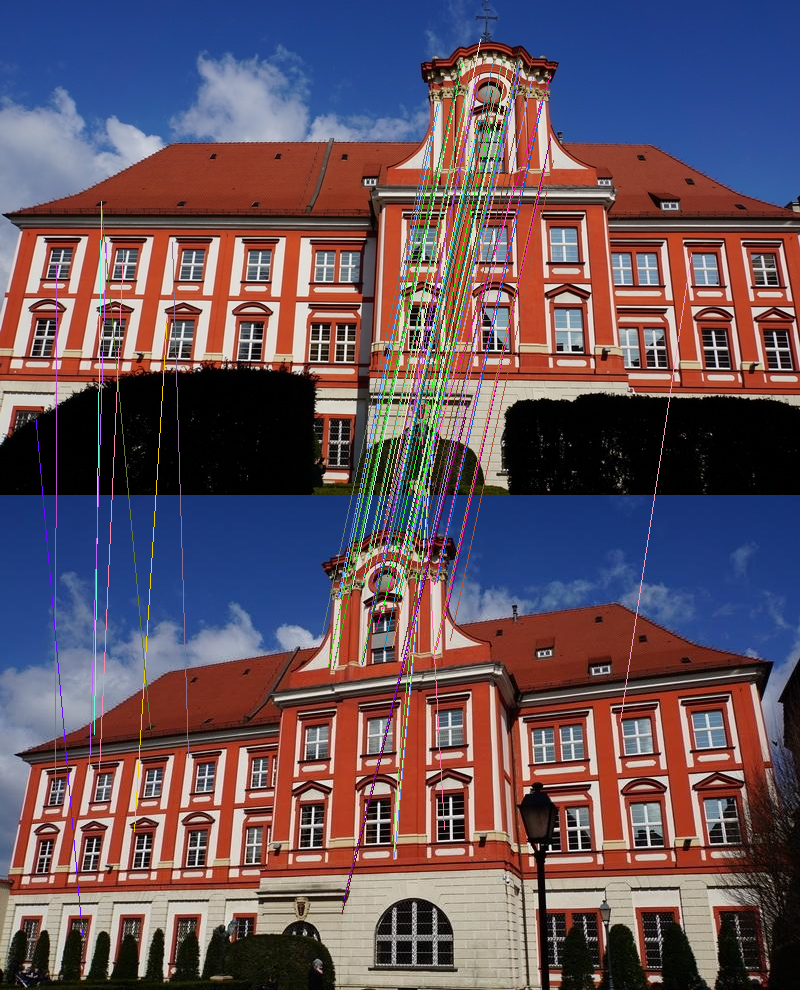
\includegraphics[width=\linewidth]{c05.png}
			\caption{c=0.5}
		\end{subfigure}
		\begin{subfigure}[b]{0.4\linewidth}
			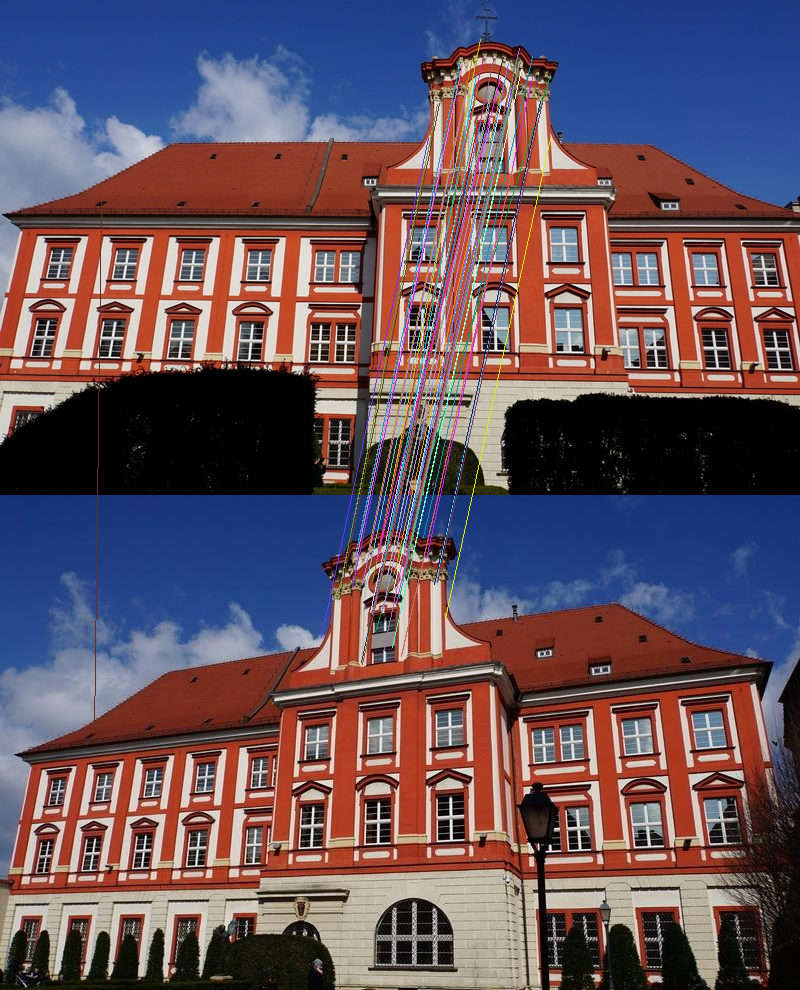
\includegraphics[width=\linewidth]{c06.png}
			\caption{c=0.6}
		\end{subfigure}
		\begin{subfigure}[b]{0.4\linewidth}
			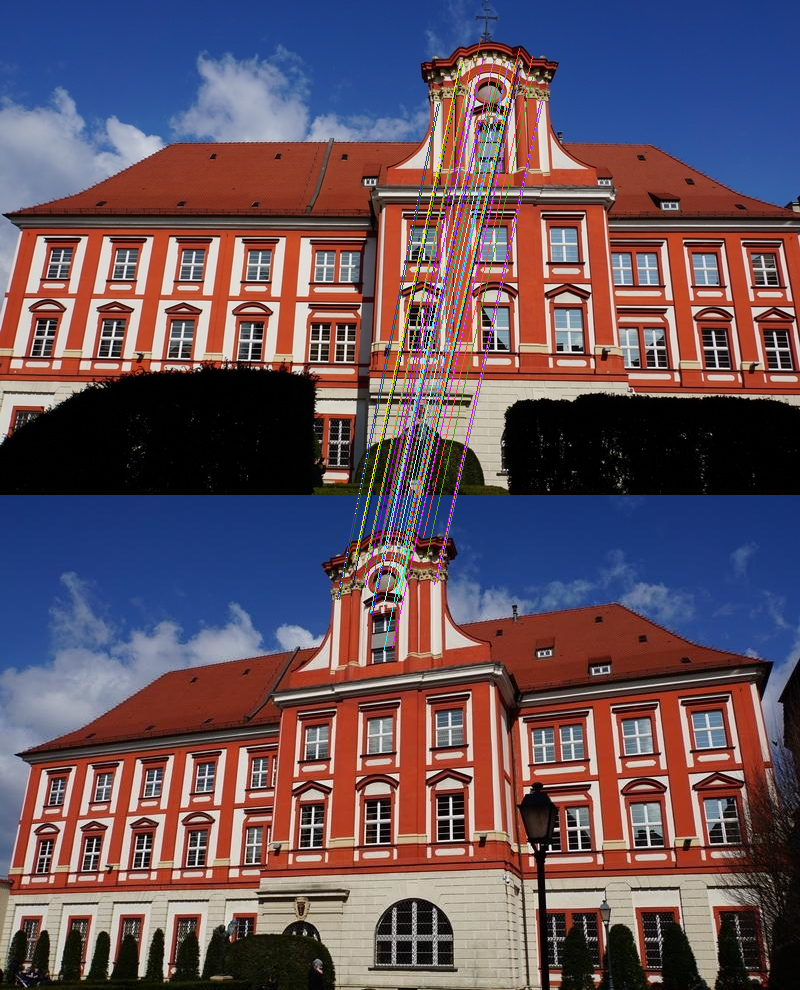
\includegraphics[width=\linewidth]{c07.png}
			\caption{c=0.7}
		\end{subfigure}
		\begin{subfigure}[b]{0.4\linewidth}
			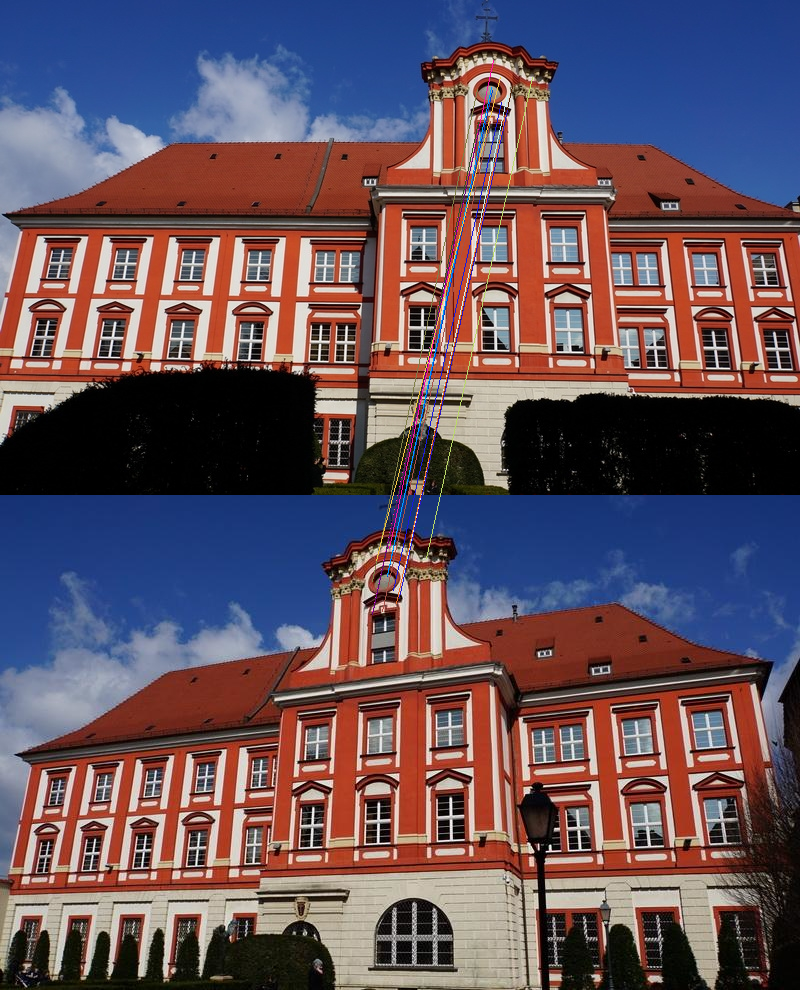
\includegraphics[width=\linewidth]{c08.png}
			\caption{c=0.8}
		\end{subfigure}
		\caption{Pary punktów kluczowych odfiltrowane za pomocą algorytmu spójności sąsiedztwa dla różnych wartości progu spójności.}
		\label{fig:cthresh}
	\end{figure}

	\begin{table}[H]
		\centering
		\caption{Porównanie liczby zaakceptowanych par punktów kluczowych w zależności od wartości progu spójności sąsiedztwa}
		\begin{tabular}{|r|r|}
			\hline
			\multicolumn{1}{|c|}{\textbf{Próg spójności}} & \multicolumn{1}{c|}{\textbf{Liczba par spójnych}} \\ \hline
			0.5                                           & 88                                                \\ \hline
			0.6                                           & 62                                                \\ \hline
			0.7                                           & 54                                                \\ \hline
			0.8                                           & 16                                                \\ \hline
			0.9                                           & 0                                                 \\ \hline
		\end{tabular}
	\end{table}
	
	\paragraph{Wnioski}
	Ustalenie dobrej wartości parametru wielkości sąsiedztwa jest kolejną istotną kwestią przy dobieraniu parametrów do algorytmu analizy spójności sąsiedztwa. Wartość tego parametru jest powiązana z wielkością sąsiedztwa więc wartości dla obu parametry powinny być ustalane równocześnie.
	Jak widać na rysunku \ref{fig:cthresh} zbyt małe wartości tego parametru mogą skutkować akceptowaniem par stanowiących szum. Z kolei zbyt duże wartości mogą powodować zgubienie istotnej, pod kątem analizy podobieństwa, informacji.\\
	Wpływ wielkości tego parametru na czas działania algorytmu okazał się nieznaczący.
	\subsection{Skuteczność działania metody RANSAC}
	\subsubsection{Wpływ rodzaju transformaty}
	Badania w tej sekcji zostaną przedstawione jako zestawienia wyników działania metody RANSAC na dwóch różnych obrazach przy wykorzystaniu transformaty afinicznej i transformaty perspektywicznej.\\
	Wszystkie badania w tej sekcji zostały przeprowadzone bez użycia heurystyk, z wartościami parametrów:
	\begin{itemize}
		\item liczba iteracji = 10000,
		\item próg akceptacji = 1.
	\end{itemize}
	
	\paragraph{Para obrazów bez zmiany perspektywy}
	Na tej parze obrazów, obiekt jest w obu przypadkach widoczny od frontu. Liczba wszystkich par punktów kluczowych na obrazie wynosi $371$.
	\begin{figure}[H]
		\centering
		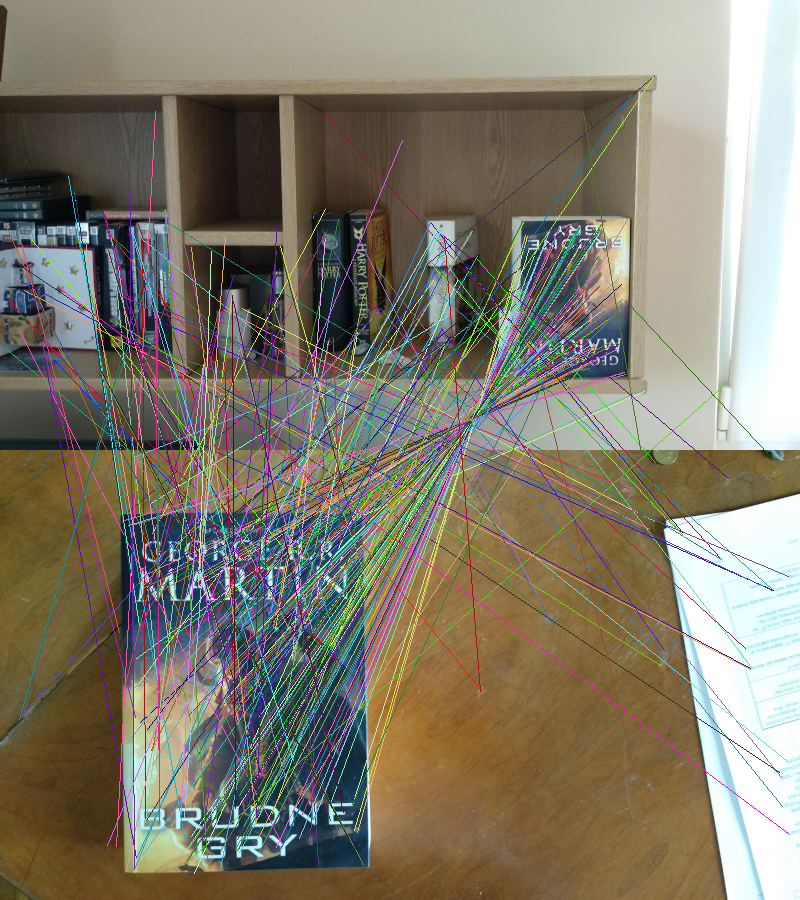
\includegraphics[width=0.6\linewidth]{all1trans.png}
		\caption{Wszystkie pary punktów kluczowych znalezione na zdjęciach książki "Brudne gry".}
	\end{figure}
	\begin{figure}[H]
		\centering
		\begin{subfigure}[b]{0.4\linewidth}
			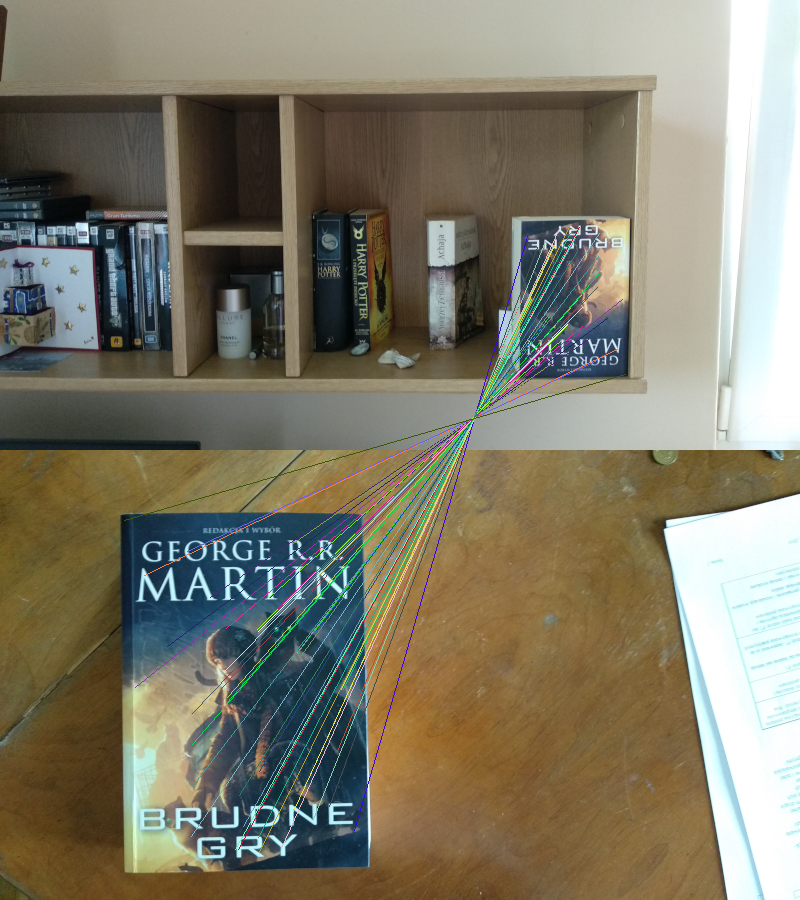
\includegraphics[width=\linewidth]{a1-match.png}
			\caption{Transformata afiniczna}
		\end{subfigure}
		\begin{subfigure}[b]{0.4\linewidth}
			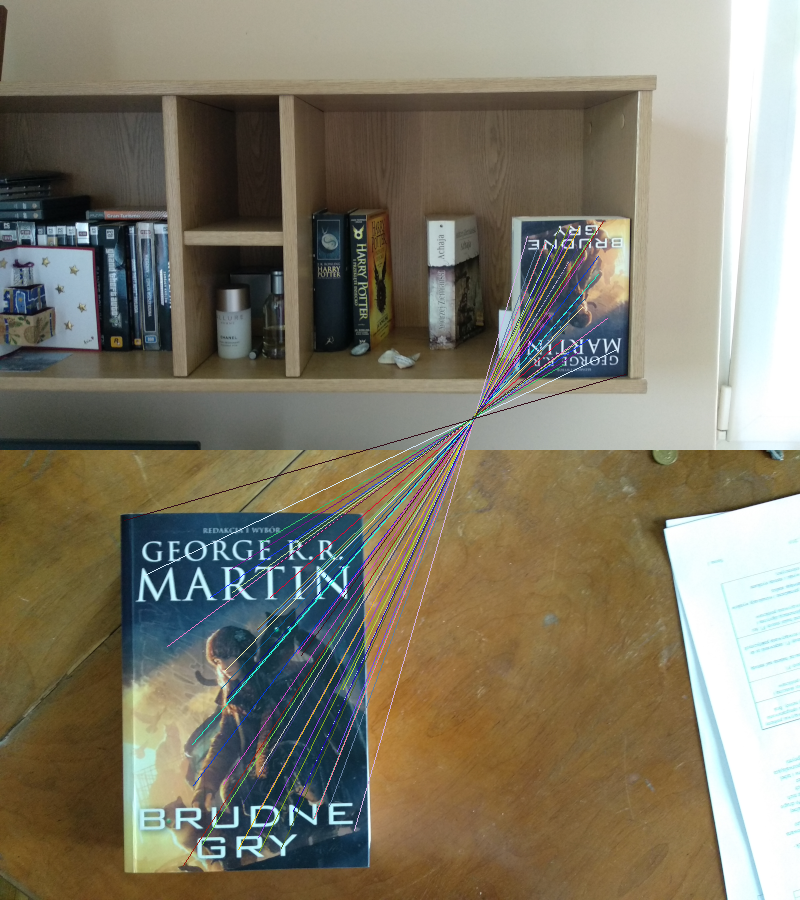
\includegraphics[width=\linewidth]{p1-match.png}
			\caption{Transformata perspektywiczna}
		\end{subfigure}
		\caption{Pary punktów kluczowych znalezione przez metodę RANSAC na zdjęciach książki "Brudne gry" przy użyciu obu przekształceń geometrycznych.}
		\label{fig:transforms11}
	\end{figure}
	\begin{figure}[H]
		\centering
		\begin{subfigure}[b]{0.4\linewidth}
			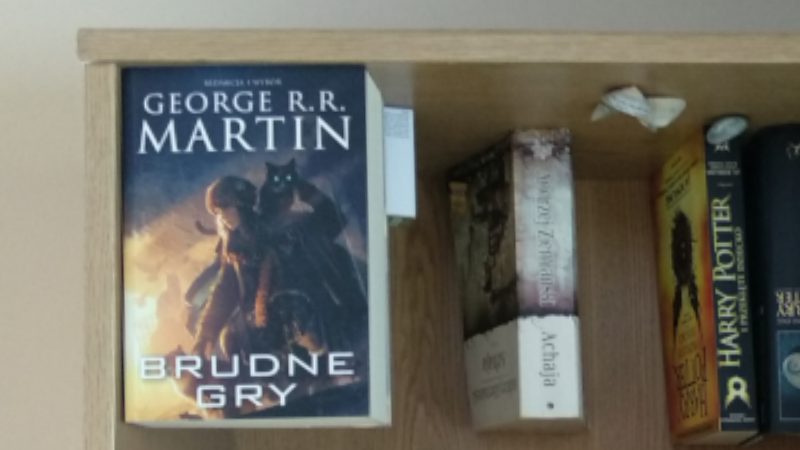
\includegraphics[width=\linewidth]{a1-trans.png}
			\caption{Transformata afiniczna}
		\end{subfigure}
		\begin{subfigure}[b]{0.4\linewidth}
			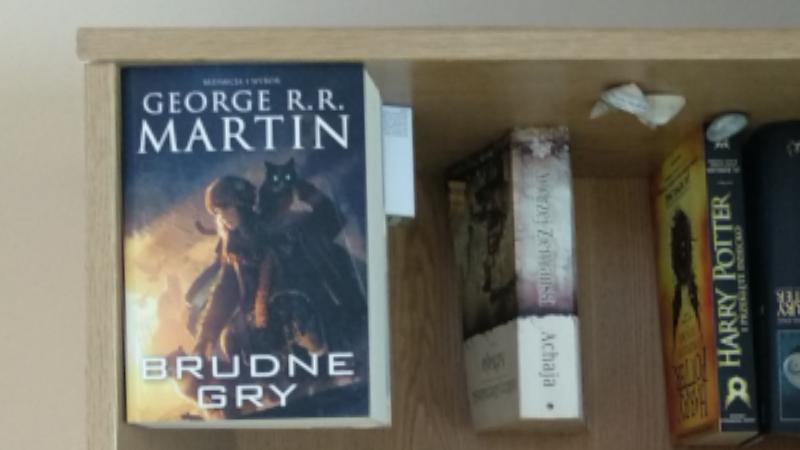
\includegraphics[width=\linewidth]{p1-trans.png}
			\caption{Transformata perspektywiczna}
		\end{subfigure}
		\caption{Najlepsze znalezione przekształcenia geometryczne zaaplikowane do całego pierwszego zdjęcia.}
		\label{fig:transforms12}
	\end{figure}

	

	\paragraph{Para obrazów ze zmianą perspektywy}
	Na tej parze obrazów, kąt patrzenia na obiekt się zmienia. Liczba par punktów kluczowych na obrazach wynosi $328$.
	\begin{figure}[H]
		\centering
		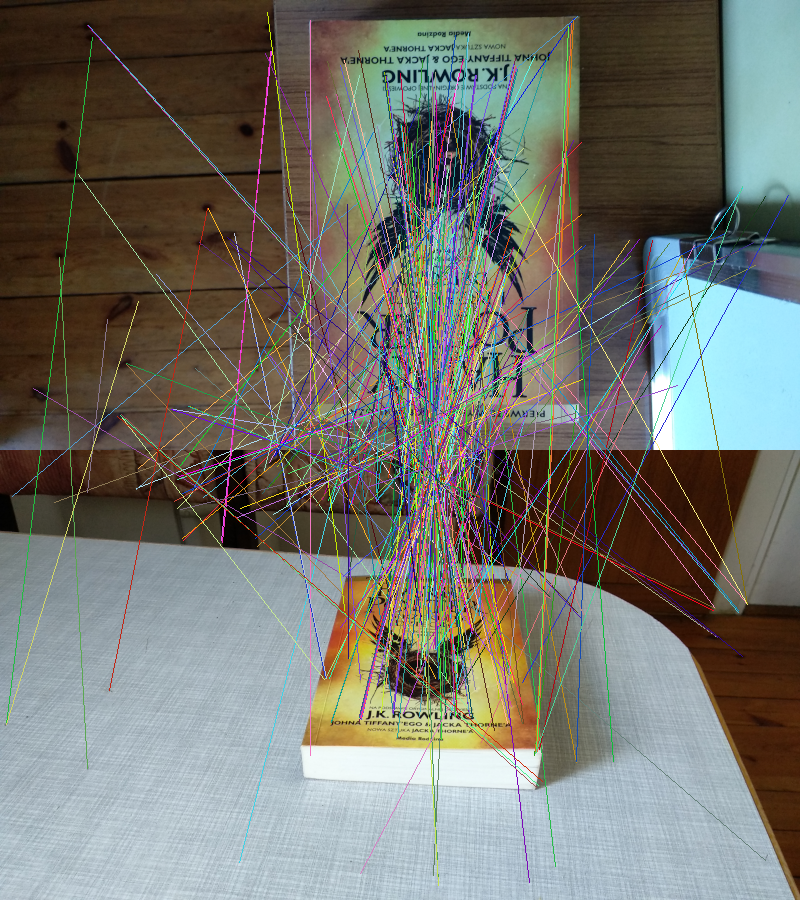
\includegraphics[width=0.6\linewidth]{all2trans.png}
		\caption{Wszystkie pary punktów kluczowych znalezione na zdjęciach książki "Harry Potter i przeklęte dziecko".}
	\end{figure}
	\begin{figure}[H]
		\centering
		\begin{subfigure}[b]{0.4\linewidth}
			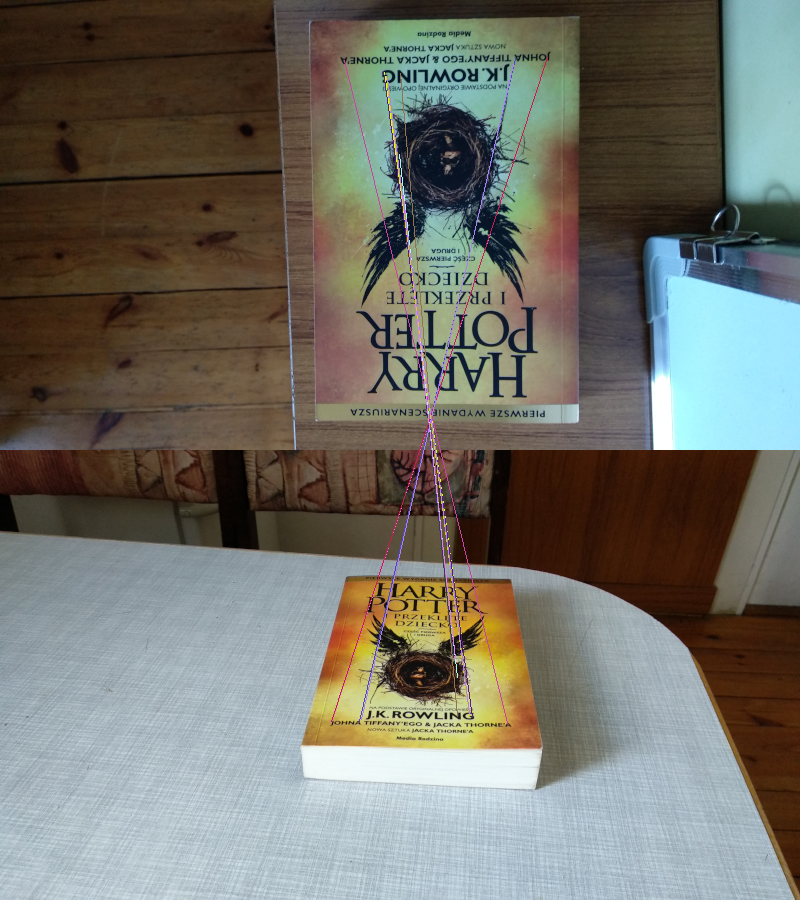
\includegraphics[width=\linewidth]{a2-match.png}
			\caption{Transformata afiniczna}
		\end{subfigure}
		\begin{subfigure}[b]{0.4\linewidth}
			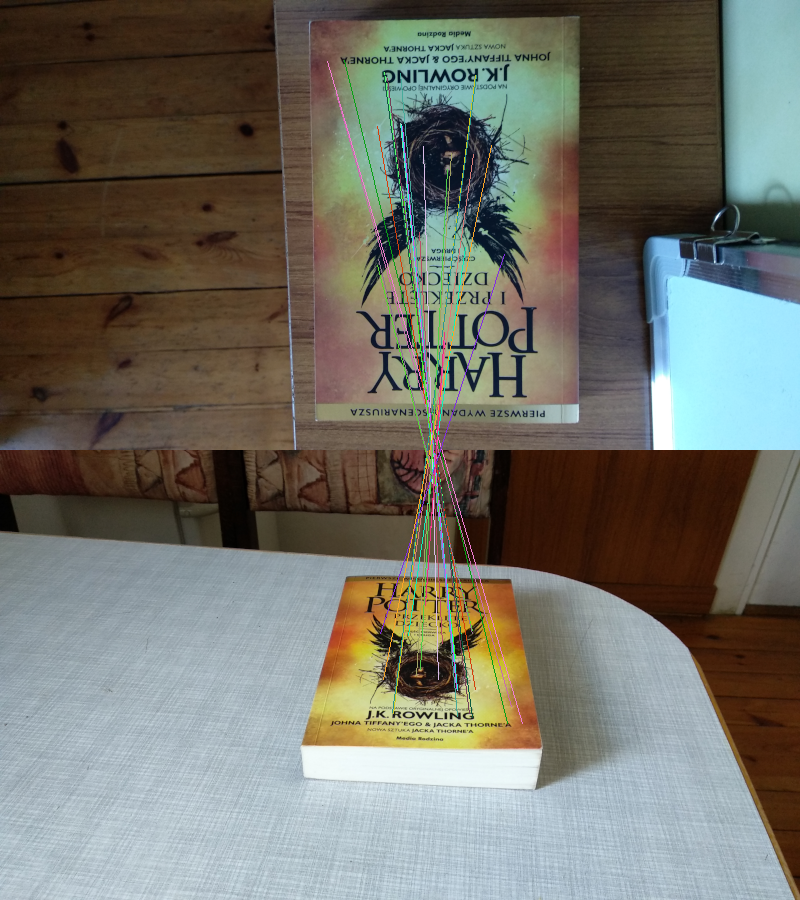
\includegraphics[width=\linewidth]{p2-match.png}
			\caption{Transformata perspektywiczna}
		\end{subfigure}
		\caption{Pary punktów kluczowych znalezione na zdjęciach książki "Harry Potter i przeklęte dziecko" przez metodę RANSAC przy użyciu obu przekształceń geometrycznych.}
		\label{fig:transforms21}
	\end{figure}
	\begin{figure}[H]
		\centering
		\begin{subfigure}[b]{0.4\linewidth}
			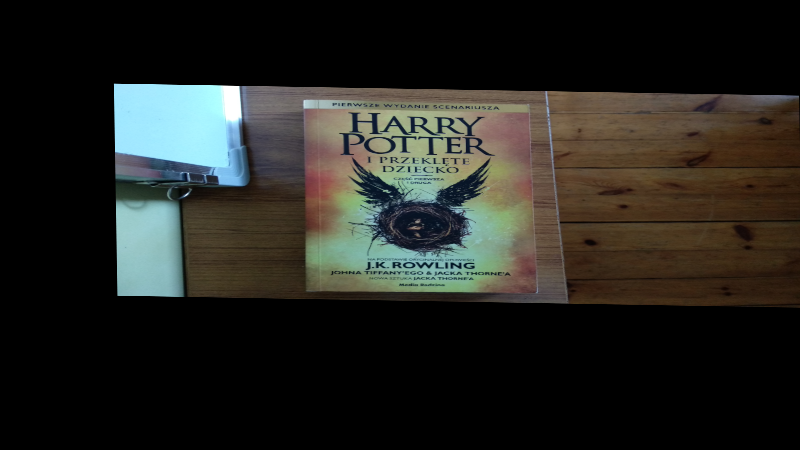
\includegraphics[width=\linewidth]{a2-trans.png}
			\caption{Transformata afiniczna}
		\end{subfigure}
		\begin{subfigure}[b]{0.4\linewidth}
			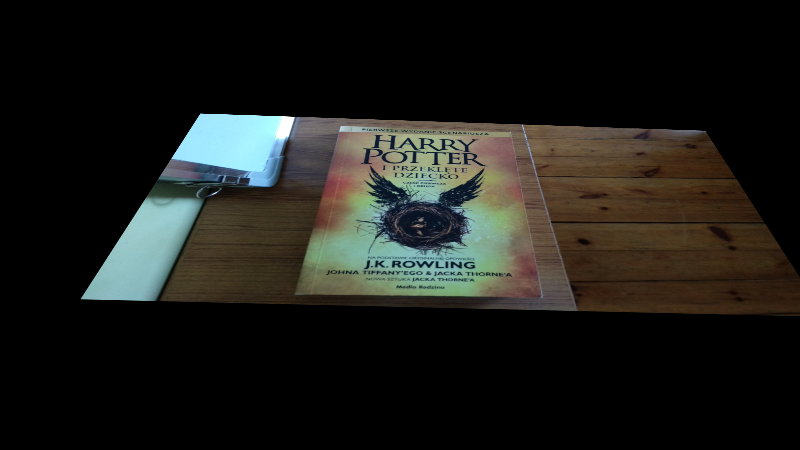
\includegraphics[width=\linewidth]{p2-trans.png}
			\caption{Transformata perspektywiczna}
		\end{subfigure}
		\caption{Najlepsze znalezione przekształcenia geometryczne zaaplikowane do całego pierwszego zdjęcia.}
		\label{fig:transforms22}
	\end{figure}

	\begin{table}[H]
		\caption{Liczba par punktów kluczowych znalezionych przez metodę RANSAC na obrazach z perspektywą i bez perspektywy (średnia z 10 przebiegów)}
		\label{tab:transforms}
		\begin{tabular}{|l|r|r|}
			\hline
			& \textbf{Transformata afiniczna} & \textbf{Transformata perspektywiczna} \\ \hline
			Bez perspektywy & 63                     & 60                           \\ \hline
			Z perspektywą   & 17                     & 35                           \\ \hline
		\end{tabular}
	\end{table}

	\paragraph{Wnioski}
	Jak widać na rysunku \ref{fig:transforms11} i w tabeli \ref{tab:transforms} w przypadku pierwszego obrazu, obie transformacje poradziły sobie podobnie. Widać również jednak, że rozwiązanie z transformacją perspektywiczną znajduje średnio mniej par, co może być związane z większą przestrzenią poszukiwań i stałą liczbą iteracji.\\
	Na rysunkach \ref{fig:transforms21} \ref{fig:transforms22} widać jednak, że w momencie kiedy obiekt na jednym z obrazów znajduje się pod innym kątem, transformacja perspektywiczna radzi sobie zdecydowanie lepiej od afinicznej. Jest to spowodowane ograniczeniami wynikającymi wprost z modelu - transformacja afiniczna nie jest w stanie reprezentować perspektywy.
	
	\subsubsection{Wpływ liczby iteracji}
	Badanie wpływu iteracji zostało przeprowadzone na parze obrazów z rysunku \ref{fig:hp1}. Ustalone wartości parametrów to:
	\begin{itemize}
		\item próg akceptacji - 1,
		\item typ transformacji - perspektywiczna.
	\end{itemize}
	\begin{table}[H]
		\centering
		\caption{Średnia liczba par pasujących do transformacji i średni czas działania dla różnych wartości liczby iteracji}
		\label{tab:iterations}
		\begin{tabular}{|r|r|r|}
			\hline
			\multicolumn{1}{|l|}{\textbf{Liczba iteracji}} & \multicolumn{1}{l|}{\textbf{Średnia liczba pasujących par}} & \multicolumn{1}{l|}{\textbf{Średni czas{[}ms{]}}} \\ \hline
			50                                             & 257,5                                                         & \textless{}1                                      \\ \hline
			100                                            & 301,2                                                         & 1                                                 \\ \hline
			200                                            & 307,1                                                         & 2                                                 \\ \hline
			500                                            & \textbf{332,7}                                                         & 5,1                                               \\ \hline
			1000                                           & 325,75                                                        & 10,7                                              \\ \hline
		\end{tabular}
	\end{table}
	\begin{figure}[H]
		\centering
		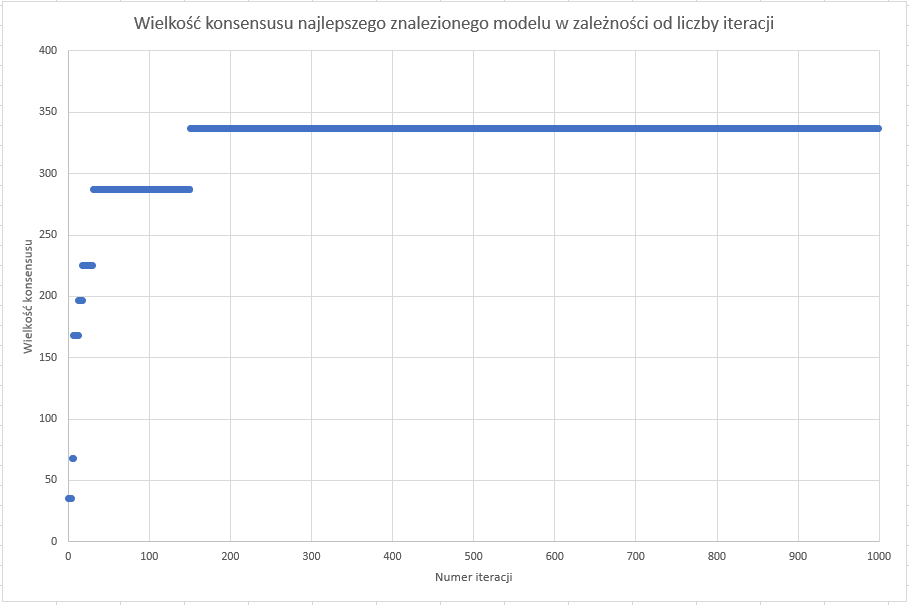
\includegraphics[width=\linewidth]{wykres1.png}
		\caption{Przykładowy przebieg metody RANSAC.}
		\label{fig:ransac_run}
	\end{figure}
	\paragraph{Wnioski}
	Liczba iteracji jest istotnym parametrem metody RANSAC, ponieważ bezpośrednio wpływa na jakość znajdowanych modeli jak i czas działania. Jak widać w tabeli \ref{tab:iterations} jak i na wykresie \ref{fig:ransac_run} istnieje pewna graniczna wartość liczby iteracji, od której zmiany wielkości są bardzo małe lub nie występują wcale. Liczbę iteracji można przez to bardzo łatwo przeszacować, powodując tym samym, że metoda będzie działać długo.

	\subsubsection{Wpływ wartości progu spójności}
	Badanie zostało przeprowadzone na tym samym obrazie co w poprzedniej sekcji. Ustalone wartości parametrów to:
	\begin{itemize}
		\item liczba iteracji - 500,
		\item typ transformacji - perspektywiczna.
	\end{itemize}

	\begin{table}[H]
		\centering
		\caption{Liczba i jakość punktów pasujących do transformacji znalezionej przez metodę RANSAC dla różnych wartości progu akceptacji}
		\label{tab:thresh}
		\begin{tabular}{|r|r|l|}
			\hline
			\multicolumn{1}{|l|}{\textbf{Próg akceptacji}} & \multicolumn{1}{l|}{\textbf{Średnia liczba par}} & \textbf{Jakość znalezionych par} \\ \hline
			1                                              & 342,5                                                           & Bardzo dobra                         \\ \hline
			5                                              & 576,3                                                           & Dobra                                \\ \hline
			20                                             & 583,2                                                           & Średnia                              \\ \hline
			50                                             & 592,7                                                           & Niska                                \\ \hline
			100                                            & 592,7                                                           & Niska                                \\ \hline
		\end{tabular}
	\end{table}
	\begin{figure}[H]
		\centering
		\begin{subfigure}[b]{0.4\linewidth}
			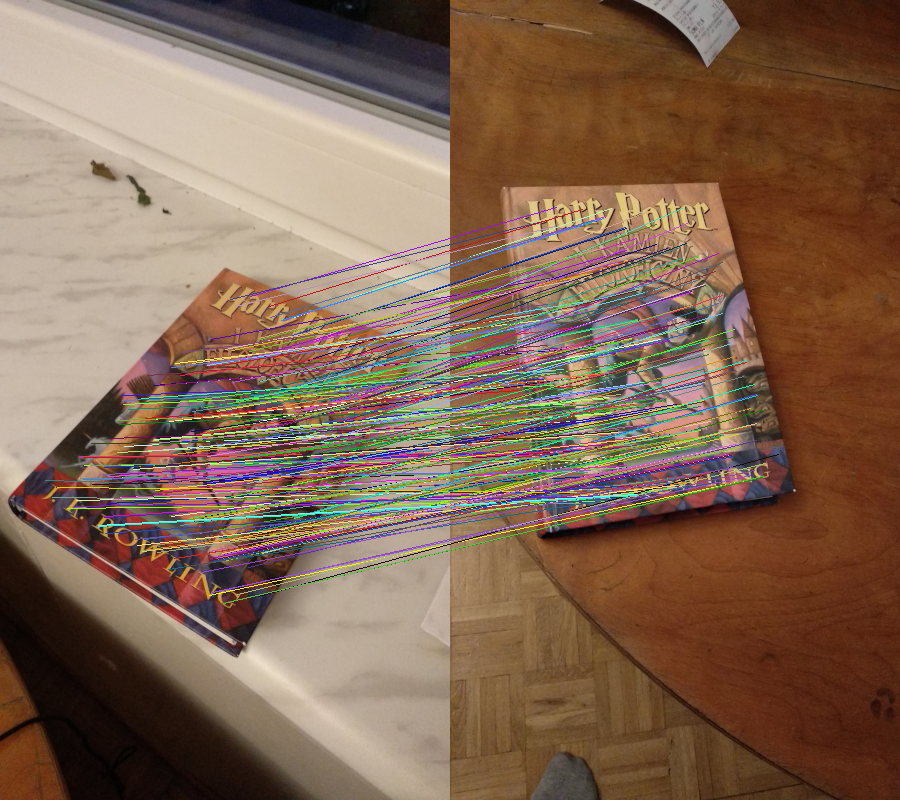
\includegraphics[width=\linewidth]{p1m.png}
			\caption{t=1}
		\end{subfigure}
		\begin{subfigure}[b]{0.4\linewidth}
			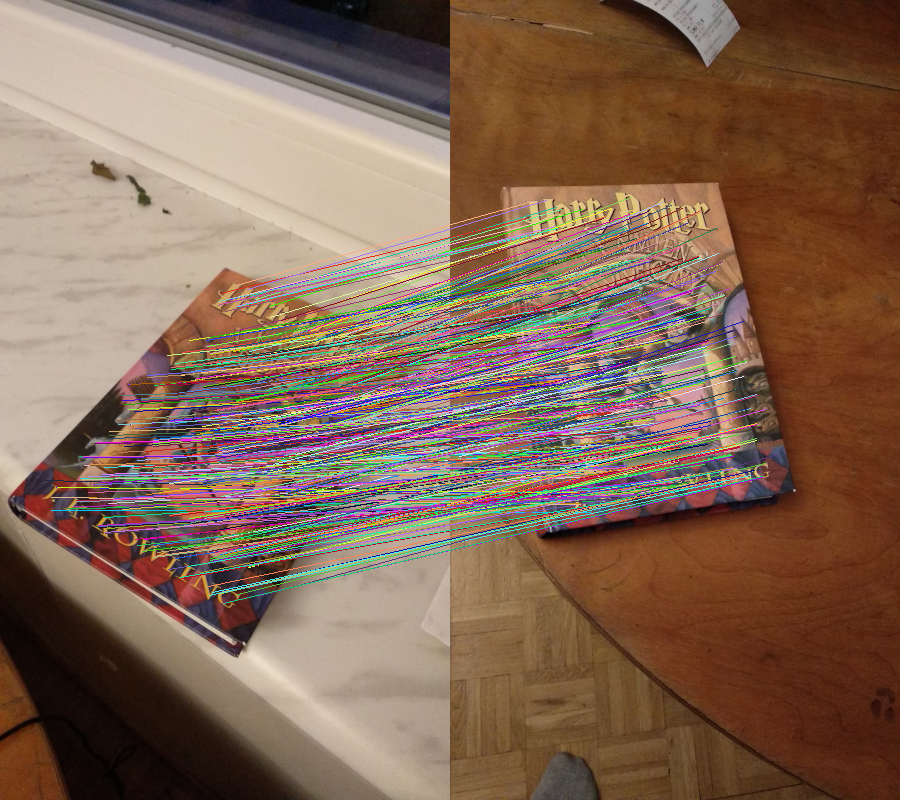
\includegraphics[width=\linewidth]{p5m.png}
			\caption{t=5}
		\end{subfigure}
		\begin{subfigure}[b]{0.4\linewidth}
			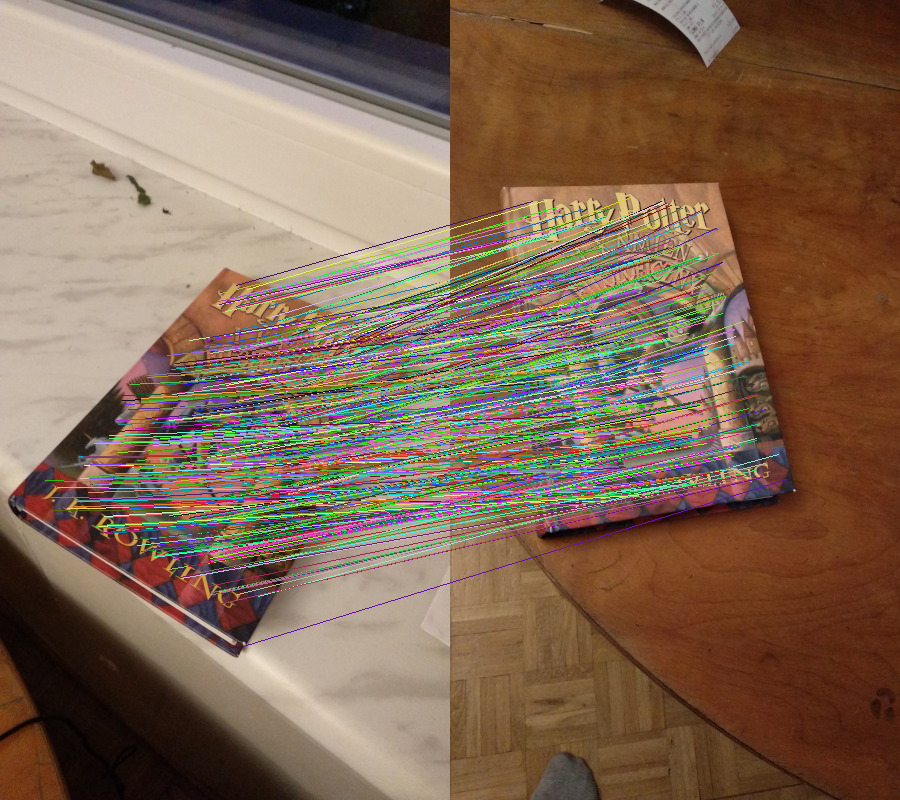
\includegraphics[width=\linewidth]{p20m.png}
			\caption{t=20}
		\end{subfigure}
		\begin{subfigure}[b]{0.4\linewidth}
			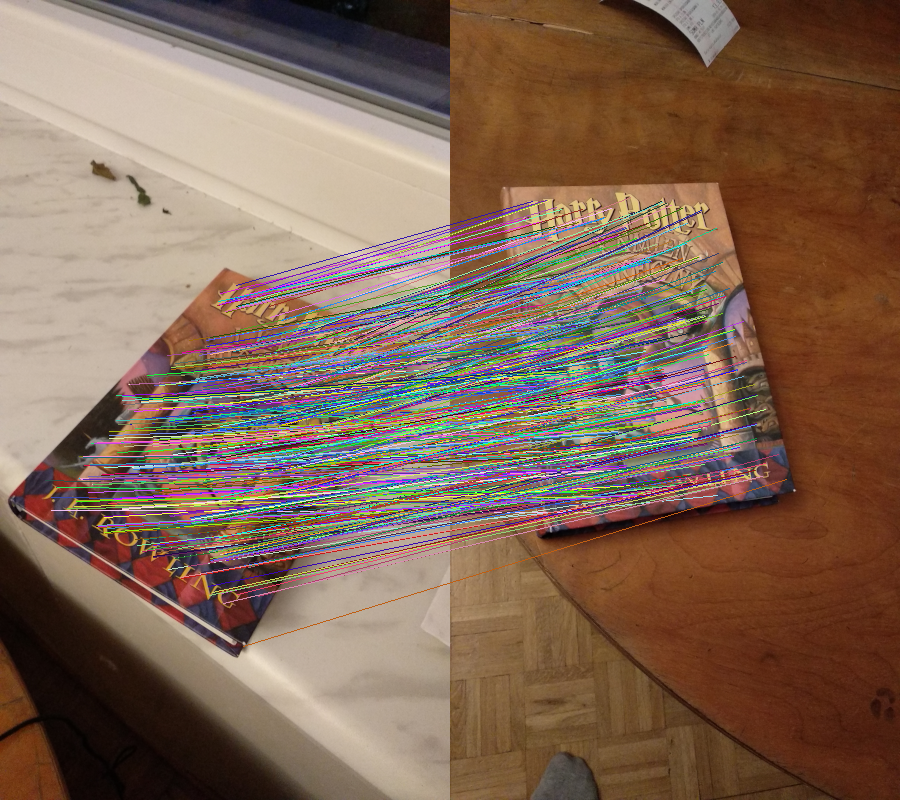
\includegraphics[width=\linewidth]{p50m.png}
			\caption{t=50}
		\end{subfigure}
		\begin{subfigure}[b]{0.4\linewidth}
			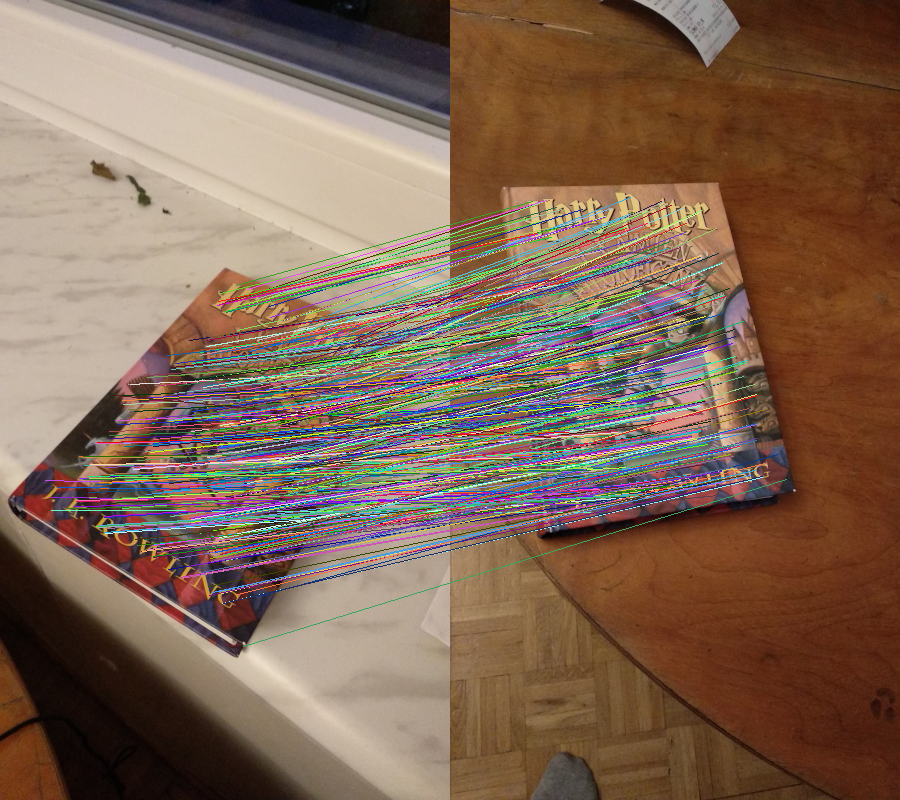
\includegraphics[width=\linewidth]{p100m.png}
			\caption{t=100}
		\end{subfigure}
		\caption{Pary punktów kluczowych pasujące do transformacji znalezionej przy różnych wartościach progu akceptacji.}
		\label{fig:thresh}
	\end{figure}
	\begin{figure}[H]
		\centering
		\begin{subfigure}[b]{0.3\linewidth}
			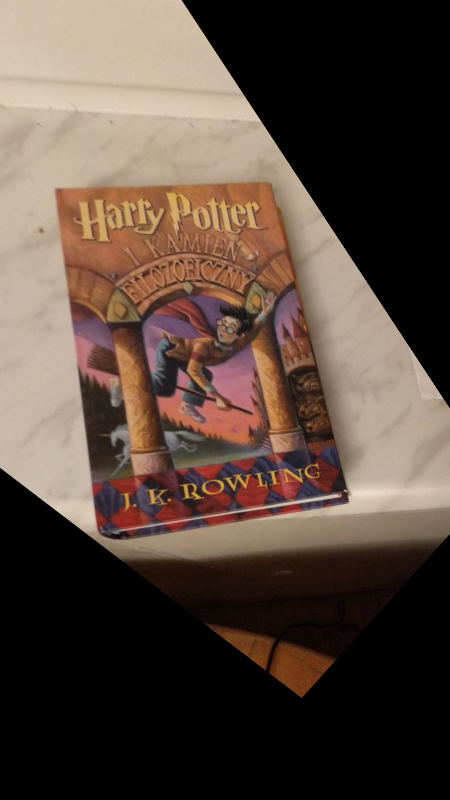
\includegraphics[width=\linewidth]{p1t.png}
			\caption{t=1}
		\end{subfigure}
		\begin{subfigure}[b]{0.3\linewidth}
			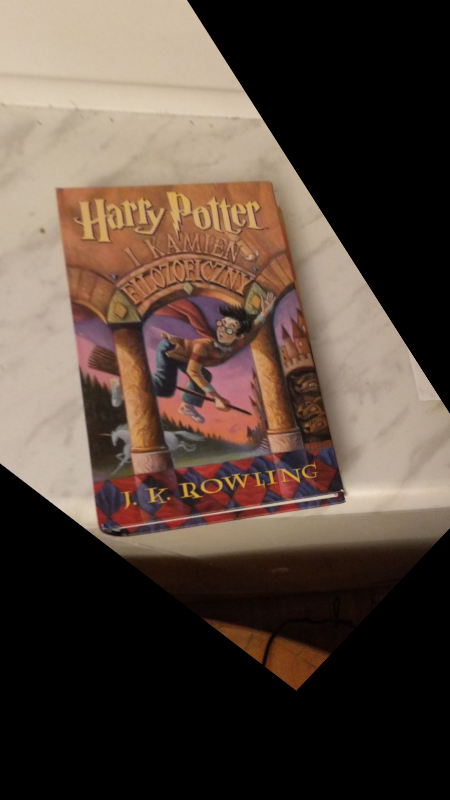
\includegraphics[width=\linewidth]{p5t.png}
			\caption{t=5}
		\end{subfigure}
		\begin{subfigure}[b]{0.3\linewidth}
			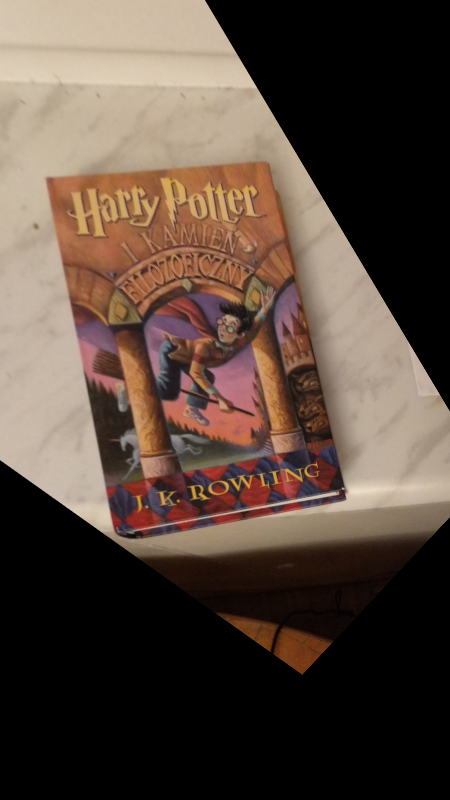
\includegraphics[width=\linewidth]{p20t.png}
			\caption{t=20}
		\end{subfigure}
		\begin{subfigure}[b]{0.3\linewidth}
			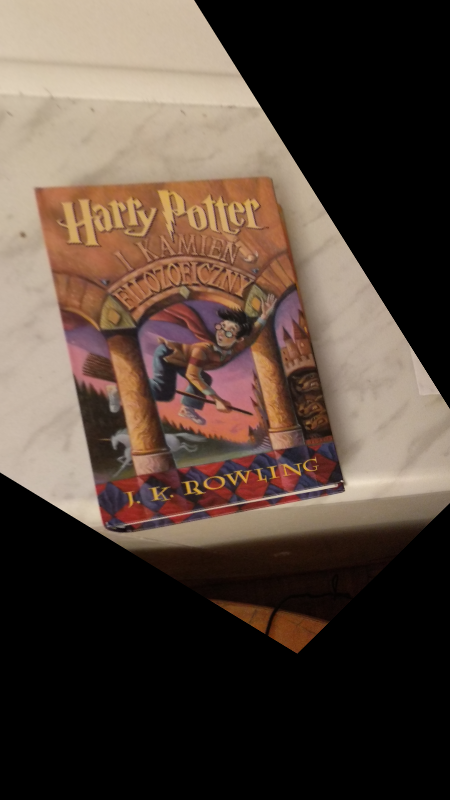
\includegraphics[width=\linewidth]{p50t.png}
			\caption{t=50}
		\end{subfigure}
		\begin{subfigure}[b]{0.3\linewidth}
			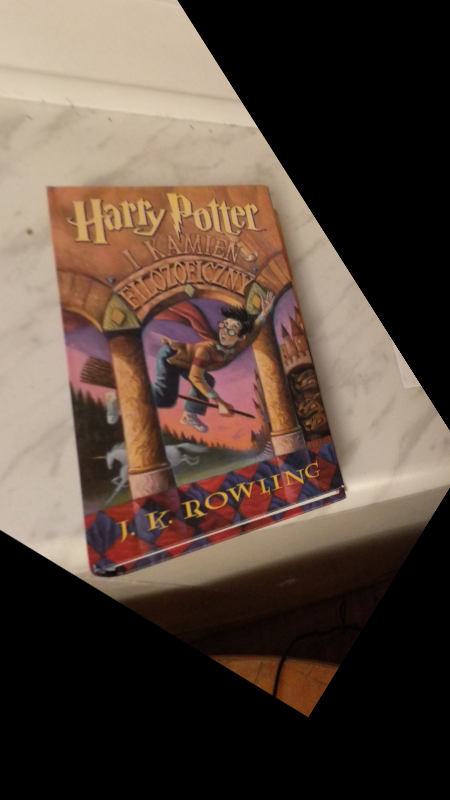
\includegraphics[width=\linewidth]{p100t.png}
			\caption{t=100}
		\end{subfigure}
		\caption{Pierwszy obraz z pary po zaaplikowaniu najlepszej znalezionej transformacji przy różnych wartościach progu akceptacji.}
		\label{fig:thresh2}
	\end{figure}
	
	\paragraph{Wnioski}
	Wartość parametru progu akceptacji danych ma istotny wpływ na jakość transformacji znajdowanych przez metodę RANSAC. Wyższe wartości tego parametru zacierają różnice pomiędzy dobrymi a słabymi modelami.
	\subsection{Heurystyki przyspieszające metodę RANSAC}
	\subsubsection{Heurystyka estymacji liczby iteracji}
	Patrząc na rysunek \ref{fig:ransac_run} można zauważyć, że po pewnej liczbie iteracji jakość modelu przestaje się poprawiać. Można więc, zamiast wybierać liczbę iteracji ręcznie, spróbować ją oszacować.
	Badania zostały przeprowadzone na zdjęciach z rysunku \ref{fig:hp1} przy następujących parametrach:
	\begin{itemize}
		\item próg spójności sąsiedztwa - 0.8,
		\item wielkość sąsiedztwa - 150.
	\end{itemize}
	
	\begin{figure}[H]
		\centering
		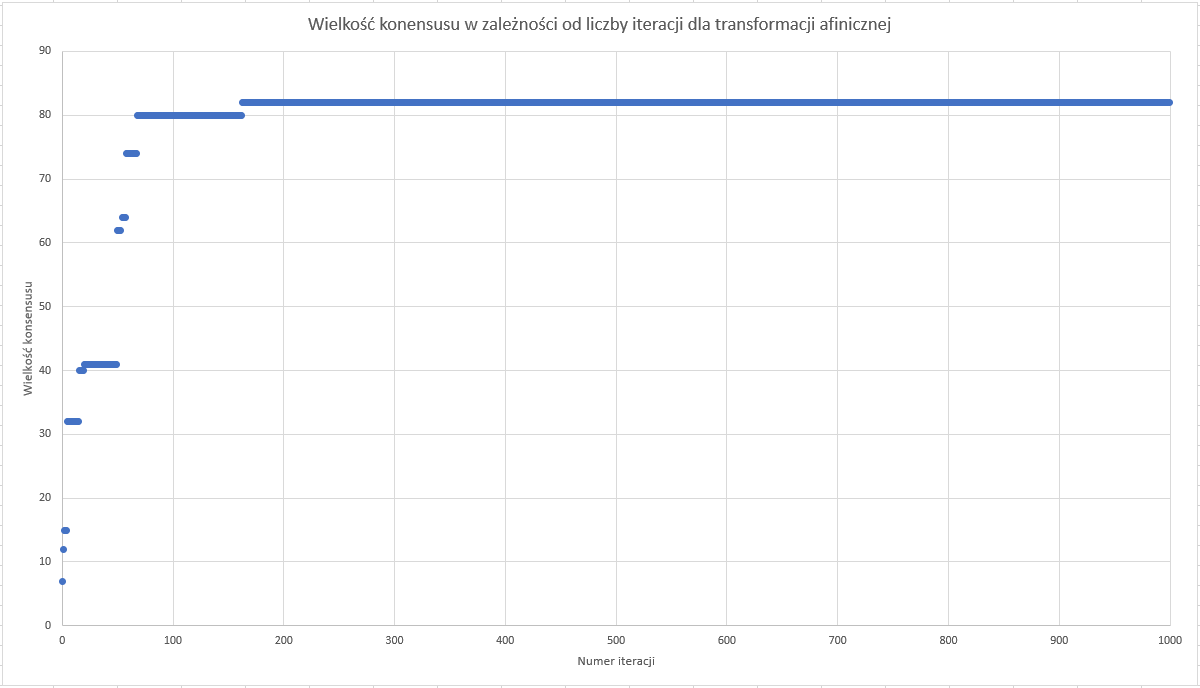
\includegraphics[width=\linewidth]{affineh.png}
		\caption{Przebieg metody RANSAC dla 1000 iteracji i transformacji afinicznej.}
		\label{fig:affineh}
	\end{figure}
	\begin{figure}[H]
		\centering
		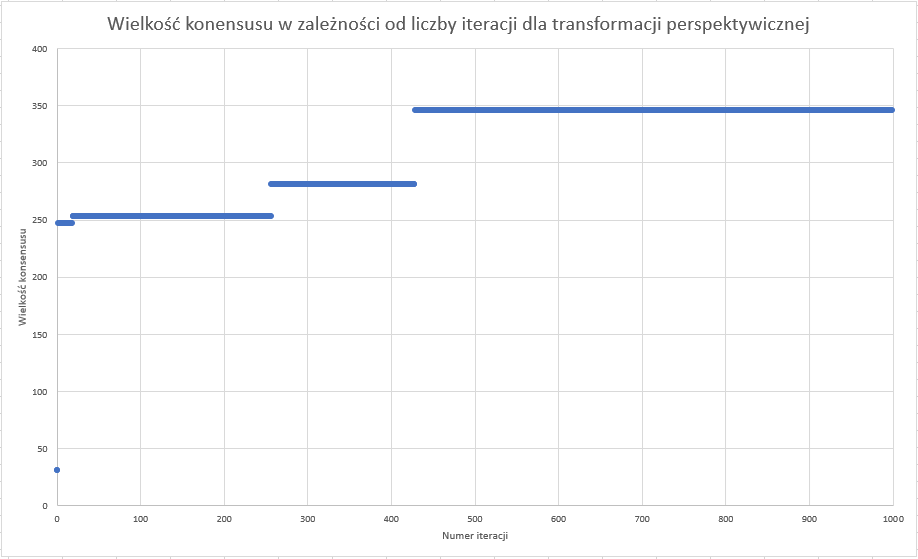
\includegraphics[width=\linewidth]{persph.png}
		\caption{Przebieg metody RANSAC dla 1000 iteracji i transformacji perspektywicznej.}
		\label{fig:persph}
	\end{figure}
	\begin{table}[H]
		\caption{Szacowane liczby iteracji w zależności od zadanego prawdopodobieństwa sukcesu dla transformacji afinicznej i perspektywicznej.}
		\centering
		\label{tab:heur_iters}
		\begin{tabular}{|r|r|r|}
			\hline
			\multicolumn{1}{|l|}{\textbf{P}} & \multicolumn{1}{l|}{\textbf{Transformacja afiniczna}} & \multicolumn{1}{l|}{\textbf{Transformacja perspektywiczna}} \\ \hline
			0.5                              & 32                                                    & 119                                                         \\ \hline
			0.6                              & 43                                                    & 158                                                         \\ \hline
			0.7                              & 57                                                    & 208                                                         \\ \hline
			0.8                              & 72                                                    & 279                                                         \\ \hline
			0.9                              & 108                                                   & 399                                                         \\ \hline
			0.99                             & 217                                                   & 800                                                         \\ \hline
		\end{tabular}
	\end{table}
	\paragraph{Wnioski}
	Jak widać z rysunków \ref{fig:affineh} i \ref{fig:persph} oraz tabeli \ref{tab:heur_iters}, gdy zadana wartość prawdopodobieństwa zbliża się do 1, wtedy oszacowana liczba iteracji zaczyna odpowiadać faktycznej liczbie iteracji wymaganej do osiągnięcia dobrego modelu. Należy jednak pamiętać, że aby użyć tej heurystyki należy również oszacować prawdopodobieństwo wystąpienia szumu na obrazie. Prowadzi to do konieczności użycia innej metody i ustalenia dobrych parametrów dla niej.
	
	\subsubsection{Heurystyka odległości}
	Badanie tej heurystyki zostało przeprowadzone na zdjęciach z rysunku \ref{fig:kubek}.
	Wartości użytych parametrów to:
	\begin{itemize}
		\item rodzaj transformacji - perspektywiczna,
		\item próg akceptacji - 1.
	\end{itemize}

	\begin{figure}[H]
		\centering
		\begin{subfigure}[b]{0.35\linewidth}
			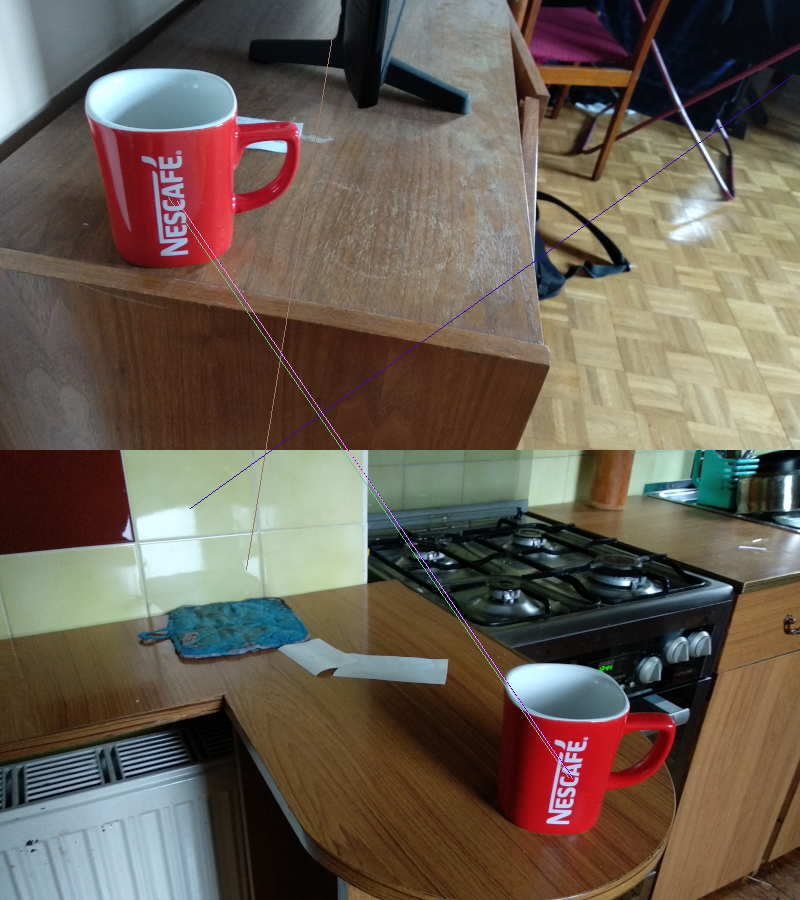
\includegraphics[width=\linewidth]{100m1.png}
			\caption{i=100, bez heurystyki}
		\end{subfigure}
		\begin{subfigure}[b]{0.35\linewidth}
			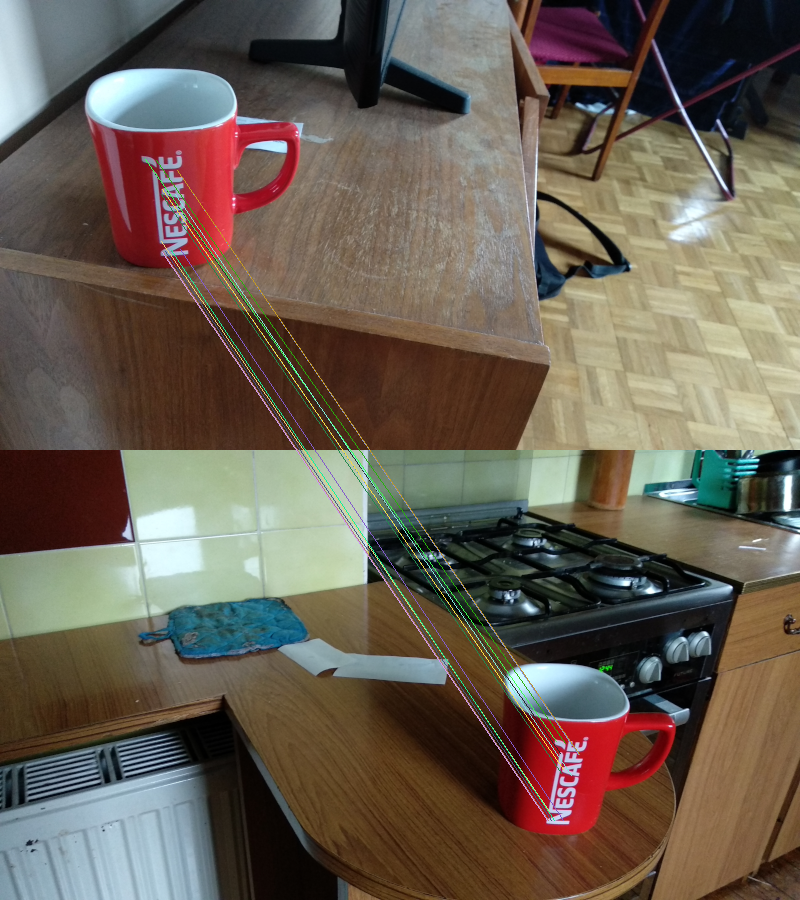
\includegraphics[width=\linewidth]{100m2.png}
			\caption{i=100, z heurystyką}
		\end{subfigure}
		\begin{subfigure}[b]{0.35\linewidth}
			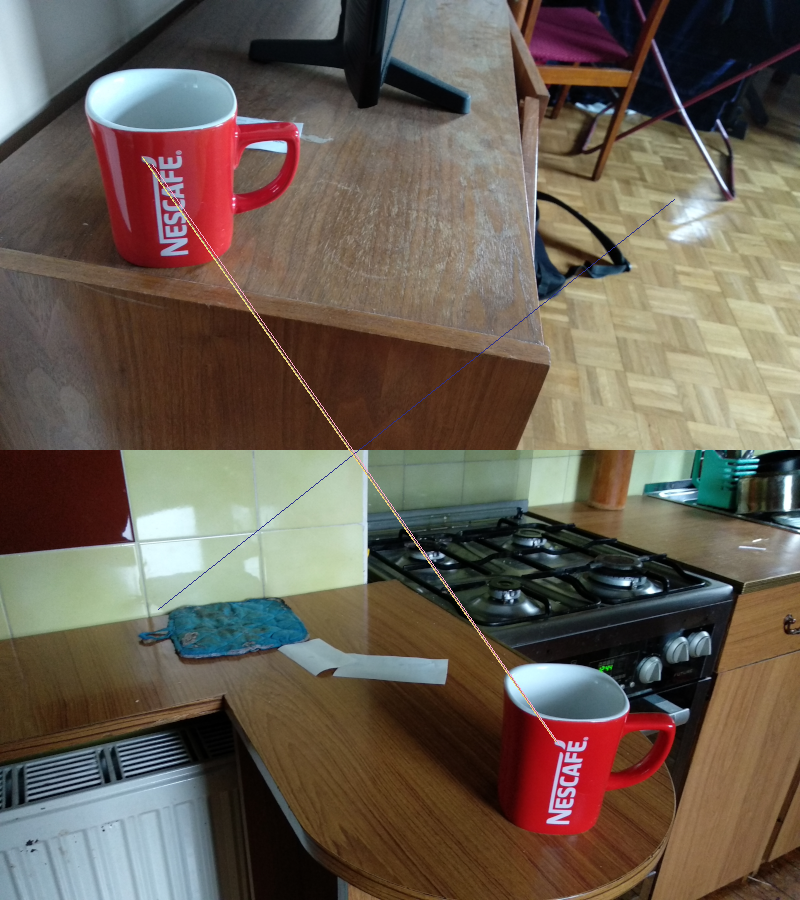
\includegraphics[width=\linewidth]{200m1.png}
			\caption{i=200, bez heurystyki}
		\end{subfigure}
		\begin{subfigure}[b]{0.35\linewidth}
			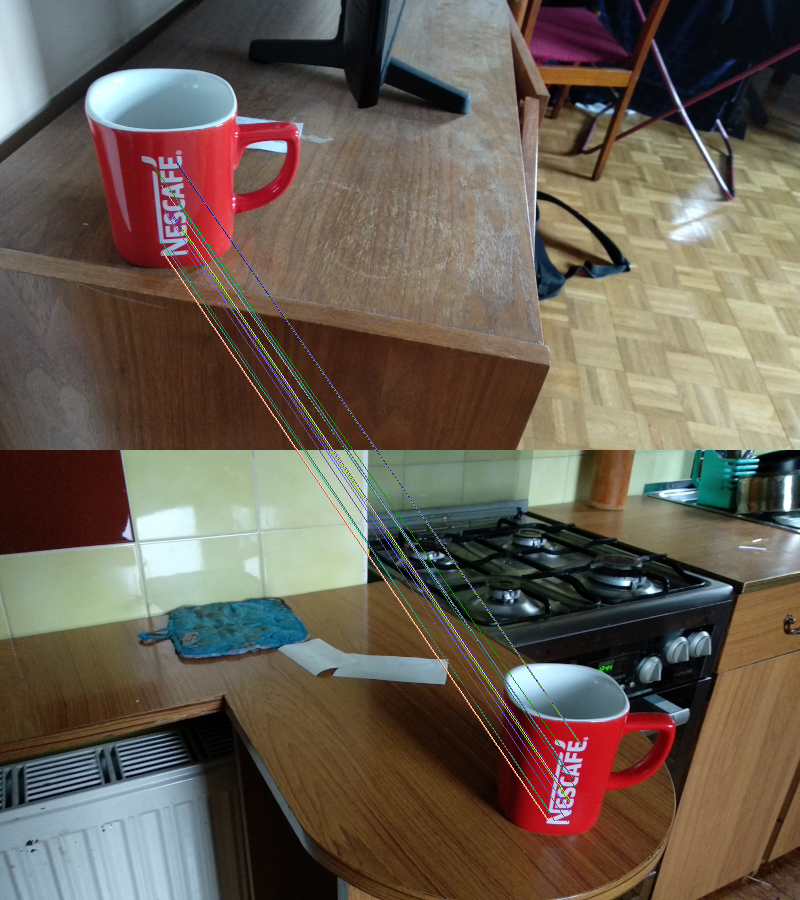
\includegraphics[width=\linewidth]{200m2.png}
			\caption{i=200, z heurystyką}
		\end{subfigure}
		\begin{subfigure}[b]{0.35\linewidth}
			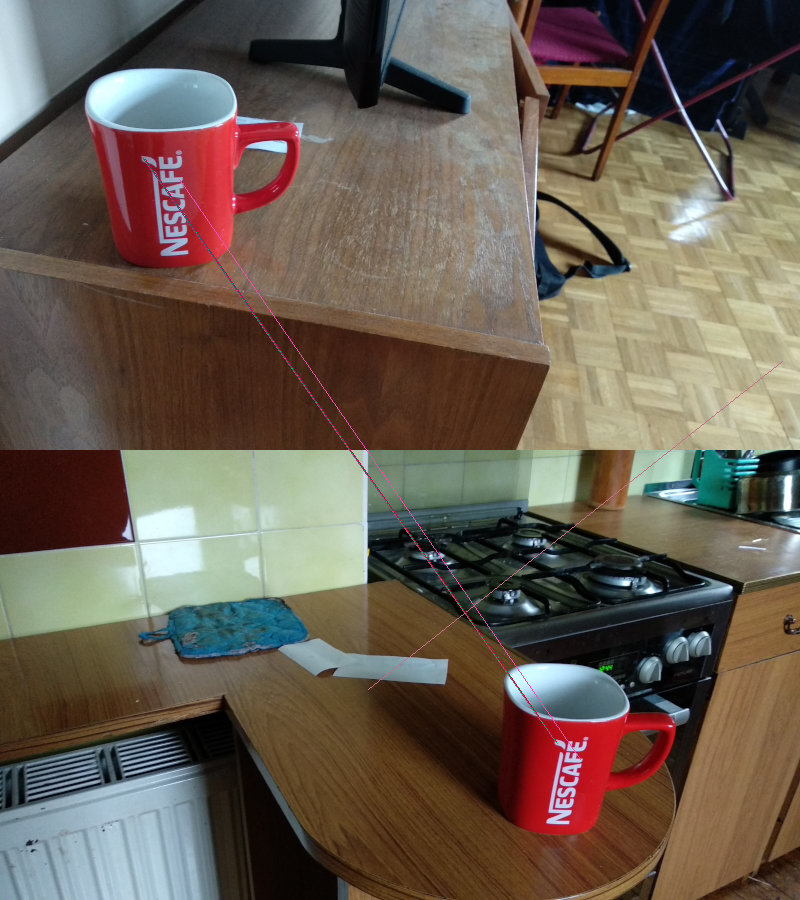
\includegraphics[width=\linewidth]{300m1.png}
			\caption{i=300, bez heurystyki}
		\end{subfigure}
		\begin{subfigure}[b]{0.35\linewidth}
			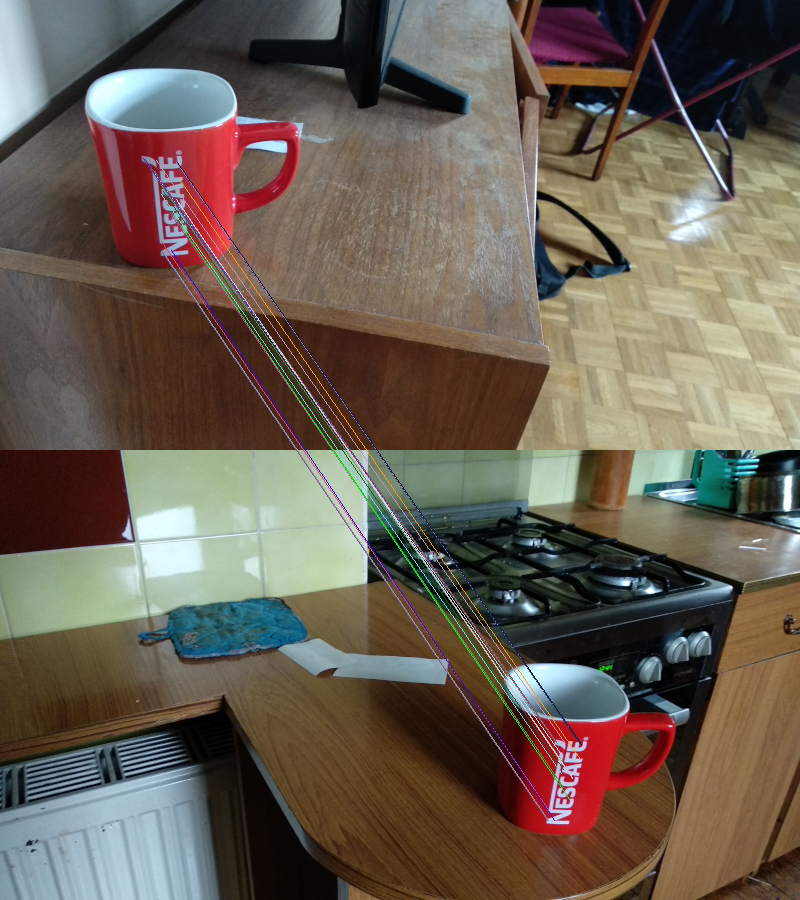
\includegraphics[width=\linewidth]{300m2.png}
			\caption{i=300, z heurystyką}
		\end{subfigure}
		\caption{Porównanie pasujących par punktów znalezionych bez heurystyki i z zastosowaną heurystyką odległości.}
			\label{fig:h2}
	\end{figure}
	\begin{figure}[H]
		\centering
		\begin{subfigure}[b]{0.35\linewidth}
			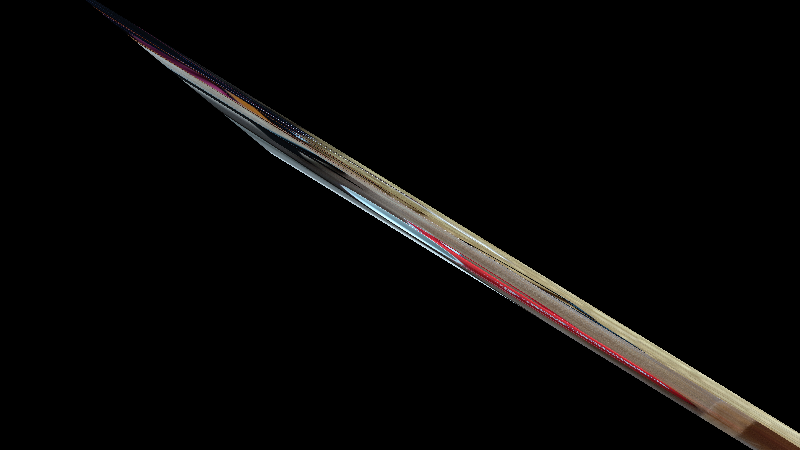
\includegraphics[width=\linewidth]{100t1.png}
			\caption{i=100, bez heurystyki}
		\end{subfigure}
		\begin{subfigure}[b]{0.35\linewidth}
			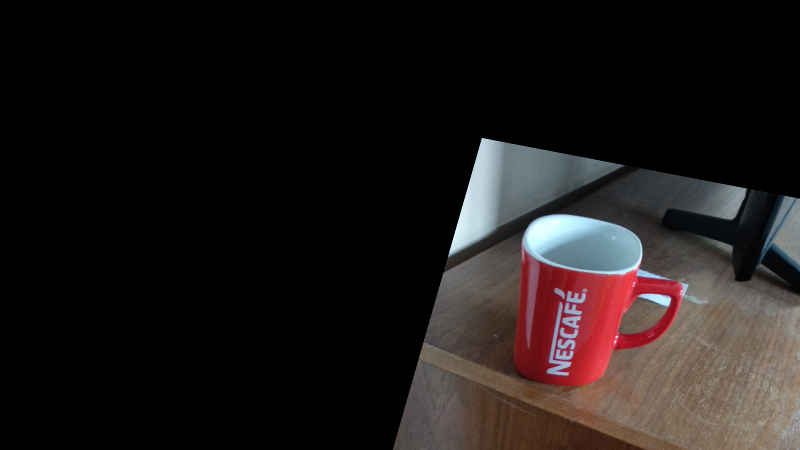
\includegraphics[width=\linewidth]{100t2.png}
			\caption{i=100, z heurystyką}
		\end{subfigure}
		\begin{subfigure}[b]{0.35\linewidth}
			\includegraphics[width=\linewidth]{200t1.png}
			\caption{i=200, bez heurystyki}
		\end{subfigure}
		\begin{subfigure}[b]{0.35\linewidth}
			\includegraphics[width=\linewidth]{200t2.png}
			\caption{i=200, z heurystyką}
		\end{subfigure}
		\begin{subfigure}[b]{0.35\linewidth}
			\includegraphics[width=\linewidth]{300t1.png}
			\caption{i=300, bez heurystyki}
		\end{subfigure}
		\begin{subfigure}[b]{0.35\linewidth}
			\includegraphics[width=\linewidth]{300t2.png}
			\caption{i=300, z heurystyką}
		\end{subfigure}
		\caption{Porównanie najlepszych transformacji znalezionych bez heurystyki i z zastosowaną heurystyką odległości.}
		\label{fig:h2transform}
	\end{figure}
	\paragraph{Wnioski}
	Jak widać na rysunkach \ref{fig:h2} i \ref{fig:h2transform} heurystyka odległości działa bardzo dobrze i pozwala znajdować jakościowo dobre przekształcenia w dużo mniejszej liczbie iteracji.
	Wpływ heurystyki na \textbf{czas przetwarzania} jest rzędu 1ms i jest pomijalny.
	
	\subsubsection{Heurystyka modyfikacji rozkładu}
	Badanie tej heurystyki zostało przeprowadzone przeprowadzone na zdjęciach z rysunku \ref{fig:kubek}.
	\begin{table}[H]
		\centering
		\caption{Srednia (10 przebiegów) liczba par znajdowanych na obrazie bez i z zastosowaną heurystyką modyfikacji rozkładu}
		\label{tab:h3}
		\begin{tabular}{|r|r|r|}
			\hline
			\multicolumn{1}{|l|}{\textbf{Liczba iteracji}} & \multicolumn{1}{l|}{\textbf{Bez heurystyki}} & \multicolumn{1}{l|}{\textbf{Z heurystyką}} \\ \hline
			100                                            & 6,5                                          & 6,9                                        \\ \hline
			500                                            & 10,3                                         & 11,1                                       \\ \hline
			1000                                           & 13,2                                         & 13,2                                       \\ \hline
			2000                                           & 12,9                                         & 15,2                                       \\ \hline
		\end{tabular}
	\end{table}
	\paragraph{Wnioski}
	Jak widać w tabeli \ref{tab:h3} heurystyka modyfikacji rozkładu nie ma tak dużego wpływu na liczbę par znajdowanych przez metodę RANSAC jak wcześniej opisane heurystyki.
	\section{Podsumowanie}
	Zarówno algorytm analizy spójności sąsiedztwa jak i zastosowanie metody RANSAC do badania podobieństwa obrazów wydaje się być sensowne. Z przeprowadzonych badań wynika jednak, że najprawdopodobniej najlepszym wyjściem byłoby zastosowanie metody RANSAC wraz z heurystyką estymacji liczby iteracji oraz heurystyką odległości, ze względu na dobre wyniki i stosunkowo niewielką liczbę parametrów do strojenia.
	\section{Profilowanie kodu}
	\begin{figure}[H]
		\centering
		\includegraphics[width=\linewidth]{before.png}
		\caption{Metoda featureDistance przed profilowaniem kodu}
		\label{fig:before1}
	\end{figure}
	\begin{figure}[H]
		\centering
		\includegraphics[width=\linewidth]{after1.png}
		\caption{Metoda featureDistance po profilowaniu kodu}
		\label{fig:after1}
	\end{figure}
	\begin{figure}[H]
		\centering
		\includegraphics[width=\linewidth]{before3.png}
		\caption{Metoda getClosest przed profilowaniem kodu}
		\label{fig:before2}
	\end{figure}
	\begin{figure}[H]
		\centering
		\includegraphics[width=\linewidth]{after3.png}
		\caption{Metoda getClosest po profilowaniu kodu}
		\label{fig:after2}
	\end{figure}
\end{document}